% Options for packages loaded elsewhere
\PassOptionsToPackage{unicode}{hyperref}
\PassOptionsToPackage{hyphens}{url}
\PassOptionsToPackage{dvipsnames,svgnames,x11names}{xcolor}
%
\documentclass[
]{article}
\usepackage{amsmath,amssymb}
\usepackage{lmodern}
\usepackage{iftex}
\ifPDFTeX
  \usepackage[T1]{fontenc}
  \usepackage[utf8]{inputenc}
  \usepackage{textcomp} % provide euro and other symbols
\else % if luatex or xetex
  \usepackage{unicode-math}
  \defaultfontfeatures{Scale=MatchLowercase}
  \defaultfontfeatures[\rmfamily]{Ligatures=TeX,Scale=1}
\fi
% Use upquote if available, for straight quotes in verbatim environments
\IfFileExists{upquote.sty}{\usepackage{upquote}}{}
\IfFileExists{microtype.sty}{% use microtype if available
  \usepackage[]{microtype}
  \UseMicrotypeSet[protrusion]{basicmath} % disable protrusion for tt fonts
}{}
\makeatletter
\@ifundefined{KOMAClassName}{% if non-KOMA class
  \IfFileExists{parskip.sty}{%
    \usepackage{parskip}
  }{% else
    \setlength{\parindent}{0pt}
    \setlength{\parskip}{6pt plus 2pt minus 1pt}}
}{% if KOMA class
  \KOMAoptions{parskip=half}}
\makeatother
\usepackage{xcolor}
\IfFileExists{xurl.sty}{\usepackage{xurl}}{} % add URL line breaks if available
\IfFileExists{bookmark.sty}{\usepackage{bookmark}}{\usepackage{hyperref}}
\hypersetup{
  pdftitle={Meta-análisis de correlaciones en R},
  pdfauthor={Juan David Leongómez1},
  colorlinks=true,
  linkcolor={gray},
  filecolor={Maroon},
  citecolor={Blue},
  urlcolor={blue},
  pdfcreator={LaTeX via pandoc}}
\urlstyle{same} % disable monospaced font for URLs
\usepackage[margin=2cm]{geometry}
\usepackage{color}
\usepackage{fancyvrb}
\newcommand{\VerbBar}{|}
\newcommand{\VERB}{\Verb[commandchars=\\\{\}]}
\DefineVerbatimEnvironment{Highlighting}{Verbatim}{commandchars=\\\{\}}
% Add ',fontsize=\small' for more characters per line
\usepackage{framed}
\definecolor{shadecolor}{RGB}{48,48,48}
\newenvironment{Shaded}{\begin{snugshade}}{\end{snugshade}}
\newcommand{\AlertTok}[1]{\textcolor[rgb]{1.00,0.81,0.69}{#1}}
\newcommand{\AnnotationTok}[1]{\textcolor[rgb]{0.50,0.62,0.50}{\textbf{#1}}}
\newcommand{\AttributeTok}[1]{\textcolor[rgb]{0.80,0.80,0.80}{#1}}
\newcommand{\BaseNTok}[1]{\textcolor[rgb]{0.86,0.64,0.64}{#1}}
\newcommand{\BuiltInTok}[1]{\textcolor[rgb]{0.80,0.80,0.80}{#1}}
\newcommand{\CharTok}[1]{\textcolor[rgb]{0.86,0.64,0.64}{#1}}
\newcommand{\CommentTok}[1]{\textcolor[rgb]{0.50,0.62,0.50}{#1}}
\newcommand{\CommentVarTok}[1]{\textcolor[rgb]{0.50,0.62,0.50}{\textbf{#1}}}
\newcommand{\ConstantTok}[1]{\textcolor[rgb]{0.86,0.64,0.64}{\textbf{#1}}}
\newcommand{\ControlFlowTok}[1]{\textcolor[rgb]{0.94,0.87,0.69}{#1}}
\newcommand{\DataTypeTok}[1]{\textcolor[rgb]{0.87,0.87,0.75}{#1}}
\newcommand{\DecValTok}[1]{\textcolor[rgb]{0.86,0.86,0.80}{#1}}
\newcommand{\DocumentationTok}[1]{\textcolor[rgb]{0.50,0.62,0.50}{#1}}
\newcommand{\ErrorTok}[1]{\textcolor[rgb]{0.76,0.75,0.62}{#1}}
\newcommand{\ExtensionTok}[1]{\textcolor[rgb]{0.80,0.80,0.80}{#1}}
\newcommand{\FloatTok}[1]{\textcolor[rgb]{0.75,0.75,0.82}{#1}}
\newcommand{\FunctionTok}[1]{\textcolor[rgb]{0.94,0.94,0.56}{#1}}
\newcommand{\ImportTok}[1]{\textcolor[rgb]{0.80,0.80,0.80}{#1}}
\newcommand{\InformationTok}[1]{\textcolor[rgb]{0.50,0.62,0.50}{\textbf{#1}}}
\newcommand{\KeywordTok}[1]{\textcolor[rgb]{0.94,0.87,0.69}{#1}}
\newcommand{\NormalTok}[1]{\textcolor[rgb]{0.80,0.80,0.80}{#1}}
\newcommand{\OperatorTok}[1]{\textcolor[rgb]{0.94,0.94,0.82}{#1}}
\newcommand{\OtherTok}[1]{\textcolor[rgb]{0.94,0.94,0.56}{#1}}
\newcommand{\PreprocessorTok}[1]{\textcolor[rgb]{1.00,0.81,0.69}{\textbf{#1}}}
\newcommand{\RegionMarkerTok}[1]{\textcolor[rgb]{0.80,0.80,0.80}{#1}}
\newcommand{\SpecialCharTok}[1]{\textcolor[rgb]{0.86,0.64,0.64}{#1}}
\newcommand{\SpecialStringTok}[1]{\textcolor[rgb]{0.80,0.58,0.58}{#1}}
\newcommand{\StringTok}[1]{\textcolor[rgb]{0.80,0.58,0.58}{#1}}
\newcommand{\VariableTok}[1]{\textcolor[rgb]{0.80,0.80,0.80}{#1}}
\newcommand{\VerbatimStringTok}[1]{\textcolor[rgb]{0.80,0.58,0.58}{#1}}
\newcommand{\WarningTok}[1]{\textcolor[rgb]{0.50,0.62,0.50}{\textbf{#1}}}
\usepackage{longtable,booktabs,array}
\usepackage{calc} % for calculating minipage widths
% Correct order of tables after \paragraph or \subparagraph
\usepackage{etoolbox}
\makeatletter
\patchcmd\longtable{\par}{\if@noskipsec\mbox{}\fi\par}{}{}
\makeatother
% Allow footnotes in longtable head/foot
\IfFileExists{footnotehyper.sty}{\usepackage{footnotehyper}}{\usepackage{footnote}}
\makesavenoteenv{longtable}
\usepackage{graphicx}
\makeatletter
\def\maxwidth{\ifdim\Gin@nat@width>\linewidth\linewidth\else\Gin@nat@width\fi}
\def\maxheight{\ifdim\Gin@nat@height>\textheight\textheight\else\Gin@nat@height\fi}
\makeatother
% Scale images if necessary, so that they will not overflow the page
% margins by default, and it is still possible to overwrite the defaults
% using explicit options in \includegraphics[width, height, ...]{}
\setkeys{Gin}{width=\maxwidth,height=\maxheight,keepaspectratio}
% Set default figure placement to htbp
\makeatletter
\def\fps@figure{htbp}
\makeatother
\setlength{\emergencystretch}{3em} % prevent overfull lines
\providecommand{\tightlist}{%
  \setlength{\itemsep}{0pt}\setlength{\parskip}{0pt}}
\setcounter{secnumdepth}{5}
\newlength{\cslhangindent}
\setlength{\cslhangindent}{1.5em}
\newlength{\csllabelwidth}
\setlength{\csllabelwidth}{3em}
\newlength{\cslentryspacingunit} % times entry-spacing
\setlength{\cslentryspacingunit}{\parskip}
\newenvironment{CSLReferences}[2] % #1 hanging-ident, #2 entry spacing
 {% don't indent paragraphs
  \setlength{\parindent}{0pt}
  % turn on hanging indent if param 1 is 1
  \ifodd #1
  \let\oldpar\par
  \def\par{\hangindent=\cslhangindent\oldpar}
  \fi
  % set entry spacing
  \setlength{\parskip}{#2\cslentryspacingunit}
 }%
 {}
\usepackage{calc}
\newcommand{\CSLBlock}[1]{#1\hfill\break}
\newcommand{\CSLLeftMargin}[1]{\parbox[t]{\csllabelwidth}{#1}}
\newcommand{\CSLRightInline}[1]{\parbox[t]{\linewidth - \csllabelwidth}{#1}\break}
\newcommand{\CSLIndent}[1]{\hspace{\cslhangindent}#1}
\usepackage{float} \floatplacement{figure}{H} \usepackage[utf8]{inputenc} \usepackage{fancyhdr} \pagestyle{fancy} \lhead{Juan David Leongómez} \rhead{\textit{Meta-análisis de correlaciones en {R:} Guía práctica}} \rfoot{\footnotesize{{doi:} \href{https://doi.org/10.5281/zenodo.5640182}{10.5281/zenodo.5640182}}} \lfoot{\footnotesize{Versión 2}} \renewcommand{\abstractname}{Descripción} \usepackage[spanish]{babel} \usepackage{hanging} \usepackage{amsthm,amssymb,amsfonts} \usepackage{tikz,lipsum,lmodern} \usepackage[most]{tcolorbox} \usepackage{fontawesome5} \renewcommand\spanishtablename{Tabla} \usepackage{multirow,booktabs,setspace,caption} \DeclareCaptionLabelSeparator*{spaced}{\\[1ex]} \captionsetup[table]{labelfont=bf,textfont=it,format=plain,justification=justified, singlelinecheck=false,labelsep=spaced,skip=5pt} \captionsetup[figure]{labelfont=bf,textfont=it,format=plain,justification=justified, singlelinecheck=false,skip=5pt}
\usepackage{booktabs}
\usepackage{longtable}
\usepackage{array}
\usepackage{multirow}
\usepackage{wrapfig}
\usepackage{float}
\usepackage{colortbl}
\usepackage{pdflscape}
\usepackage{tabu}
\usepackage{threeparttable}
\usepackage{threeparttablex}
\usepackage[normalem]{ulem}
\usepackage{makecell}
\usepackage{xcolor}
\ifLuaTeX
  \usepackage{selnolig}  % disable illegal ligatures
\fi

\title{Meta-análisis de correlaciones en R}
\usepackage{etoolbox}
\makeatletter
\providecommand{\subtitle}[1]{% add subtitle to \maketitle
  \apptocmd{\@title}{\par {\large #1 \par}}{}{}
}
\makeatother
\subtitle{Guía práctica}
\author{Juan David Leongómez\textsuperscript{1}}
\date{23 febrero, 2022}

\begin{document}
\maketitle

\textsuperscript{1} Laboratorio de Análisis del Comportamiento Humano (LACH), Facultad de Psicología, Universidad El Bosque, Bogotá, Colombia. Email: \href{mailto:jleongomez@unbosque.edu.co}{\nolinkurl{jleongomez@unbosque.edu.co}}. Web: \href{https://jdleongomez.info/es/}{jdleongomez.info}.

\newtcolorbox{Box2}[2][]{
                lower separated=false,
                colback=white,
                colframe=darkgray,
                fonttitle=\bfseries,
                colbacktitle=gray,
                coltitle=white,
                boxrule=0.2pt,
                outer arc=1pt,
                breakable,
                enhanced,
                attach boxed title to top left={yshift=-0.1in,xshift=0.15in},
                boxed title style={boxrule=0pt,colframe=white,},
title=#2,#1}

\vfill
\begin{center}
\textbf{Descripción}
\end{center}

Este documento contiene todo el código explicaciones básicas, paso a paso, para hacer un meta-análisis en R, usando los paquetes \href{https://www.metafor-project.org/doku.php}{\texttt{metafor}} (\protect\hyperlink{ref-viechtbauer2010}{Viechtbauer, 2010}) y \href{https://www.rdocumentation.org/packages/robumeta}{\texttt{robumeta}} (\protect\hyperlink{ref-fisherRobumetaRpackageRobust2015}{Fisher \& Tipton, 2015}). Está principalmente basado en \href{https://youtu.be/lH4VZMTEZSc}{este video}, creado por Daniel S. Quintana (\protect\hyperlink{ref-quintanaHowPerformMetaanalysis2021}{2021}), pero contiene citas a fuentes primarias, además de información que he agregado.

Esta guía asume una comprensión básica del meta-análisis, así como un manejo básico de R. Sin embargo, de ser necesario, como introducción al meta-análisis recomiendo ver el video introductorio sobre meta-análisis en \emph{jamovi} (\protect\hyperlink{ref-leongomezMetaanalysis2021}{Leongómez, 2021}) que publiqué anteriormente en mi canal de YouTube \href{https://www.youtube.com/c/InvestigaciónAbierta}{\emph{Investigación Abierta}}.

\href{https://www.youtube.com/c/InvestigaciónAbierta}{
\includegraphics{Logo-IA-Rectangulo.png}}

\vfill

\begin{center}\rule{0.5\linewidth}{0.5pt}\end{center}

\textbf{Cita éste trabajo como:}

\begin{hangparas}{.25in}{1}
Leongómez, J. D. (2022). \textit{Meta-análisis de correlaciones en R: Guía práctica.} Zenodo. \url{https://doi.org/10.5281/zenodo.5640182}
\end{hangparas}
\newpage

{\hypersetup{hidelinks}
 \setcounter{tocdepth}{5}
 \tableofcontents
}

\begin{center}\rule{0.5\linewidth}{0.5pt}\end{center}

\hypertarget{base-de-datos-de-ejemplo}{%
\section{Base de datos de ejemplo}\label{base-de-datos-de-ejemplo}}

Para los ejemplos usados en ésta guía, usaré la base de datos \texttt{dat.molloy2014}, tomada de Molloy et al. (\protect\hyperlink{ref-molloy2013}{2013}).

Esta base de datos viene incluida con el paquete \texttt{\{metafor\}} de R. Básicamente, Molloy et al. (\protect\hyperlink{ref-molloy2013}{2013}) estudiaron si existe una asociación entre la diligencia (\emph{conscientiousness}) y la adherencia a la medicación. En otras palabras, ¿las personas más diligentes son más propensas a cumplir con la medicación prescrita?

Primero, primero, debemos cargar los paquetes que usaremos, incluyendo \texttt{\{metafor\}} y \texttt{\{robumeta\}} para hacer metaánálisis, así como \texttt{\{dplyr\}} para manipular y organizar la base de datos.

\begin{Shaded}
\begin{Highlighting}[]
\FunctionTok{library}\NormalTok{(robumeta)}
\FunctionTok{library}\NormalTok{(metafor)}
\FunctionTok{library}\NormalTok{(dplyr)}
\end{Highlighting}
\end{Shaded}

Una vez cargado el paquete \texttt{\{metafor\}}, ya puedo cargar la base de datos \texttt{dat.molloy2014}. En éste caso, para poder \emph{llamarla} cuando sea necesario, la asignaré a un objeto llamado \texttt{dat}.

\begin{Shaded}
\begin{Highlighting}[]
\NormalTok{dat }\OtherTok{\textless{}{-}} \FunctionTok{get}\NormalTok{(}\FunctionTok{data}\NormalTok{(dat.molloy2014))}
\end{Highlighting}
\end{Shaded}

Tras asignar la base de datos a este objeto (\texttt{dat}), podemos verla en la consola de R sencillamente usando el comando \texttt{dat}.

\begin{Shaded}
\begin{Highlighting}[]
\NormalTok{dat}
\end{Highlighting}
\end{Shaded}

\begin{footnotesize}
                \begin{Box2}{\texttt{Consola de R}}
                \begin{verbatim}                authors year  ni     ri controls          design   a_measure
1      Axelsson et al. 2009 109  0.187     none cross-sectional self-report
2      Axelsson et al. 2011 749  0.162     none cross-sectional self-report
3         Bruce et al. 2010  55  0.340     none     prospective       other
4   Christensen et al. 1999 107  0.320     none cross-sectional self-report
5  Christensen & Smith 1995  72  0.270     none     prospective       other
6         Cohen et al. 2004  65  0.000     none     prospective       other
7       Dobbels et al. 2005 174  0.175     none cross-sectional self-report
8        Ediger et al. 2007 326  0.050 multiple     prospective self-report
9         Insel et al. 2006  58  0.260     none     prospective       other
10       Jerant et al. 2011 771  0.010 multiple     prospective       other
11        Moran et al. 1997  56 -0.090 multiple     prospective       other
12   O'Cleirigh et al. 2007  91  0.370     none     prospective self-report
13       Penedo et al. 2003 116  0.000     none cross-sectional self-report
14        Quine et al. 2012 537  0.150     none     prospective self-report
15      Stilley et al. 2004 158  0.240     none     prospective       other
16 Wiebe & Christensen 1997  65  0.040     none     prospective       other
   c_measure meanage quality
1      other   22.00       1
2        NEO   53.59       1
3        NEO   43.36       2
4      other   41.70       1
5        NEO   46.39       2
6        NEO   41.20       2
7        NEO   52.30       1
8        NEO   41.00       3
9      other   77.00       2
10       NEO   78.60       3
11       NEO   57.20       2
12       NEO   37.90       2
13       NEO   39.20       1
14     other   69.00       2
15       NEO   46.20       3
16       NEO   56.00       1
 \end{verbatim}
                \end{Box2}
                \end{footnotesize}

Por supuesto, la salida de la consola no es la más clara, así que de aquí en adelante mostraré cualquier tabla en un formato de impresión. Voy a volver a cargar la base de datos (sobreescribiendo el objeto \texttt{dat}), para organizarla un poco mejor. Primero, agregaré una nueva columna llamada \texttt{study\_id}, en la que numeraré los estudios del 1 al 16. A continuación, reorganizaré las columnas para que \texttt{study\_id} sea la primera, en vez de la última columna.

\begin{Shaded}
\begin{Highlighting}[]
\NormalTok{dat }\OtherTok{\textless{}{-}} \FunctionTok{get}\NormalTok{(}\FunctionTok{data}\NormalTok{(dat.molloy2014)) }\SpecialCharTok{\%\textgreater{}\%}
  \FunctionTok{mutate}\NormalTok{(}\AttributeTok{study\_id =} \DecValTok{1}\SpecialCharTok{:}\DecValTok{16}\NormalTok{)  }\SpecialCharTok{\%\textgreater{}\%} \CommentTok{\#agregar columna study\_id}
  \FunctionTok{select}\NormalTok{(study\_id, authors}\SpecialCharTok{:}\NormalTok{quality) }\CommentTok{\#mover study\_id como primera columna}
\end{Highlighting}
\end{Shaded}

Con esto, la base de datos tiene ahora la siguiente estructura (Tabla \ref{tab:estructuramod}):

\begin{table}[H]

\caption{\label{tab:estructuramod}Estructura de la base de datos con estudios numerados}
\centering
\resizebox{\linewidth}{!}{
\begin{tabular}[t]{rlrrrllllrr}
\toprule
study\_id & authors & year & ni & ri & controls & design & a\_measure & c\_measure & meanage & quality\\
\midrule
1 & Axelsson et al. & 2009 & 109 & 0.187 & none & cross-sectional & self-report & other & 22.00 & 1\\
2 & Axelsson et al. & 2011 & 749 & 0.162 & none & cross-sectional & self-report & NEO & 53.59 & 1\\
3 & Bruce et al. & 2010 & 55 & 0.340 & none & prospective & other & NEO & 43.36 & 2\\
4 & Christensen et al. & 1999 & 107 & 0.320 & none & cross-sectional & self-report & other & 41.70 & 1\\
5 & Christensen \& Smith & 1995 & 72 & 0.270 & none & prospective & other & NEO & 46.39 & 2\\
6 & Cohen et al. & 2004 & 65 & 0.000 & none & prospective & other & NEO & 41.20 & 2\\
7 & Dobbels et al. & 2005 & 174 & 0.175 & none & cross-sectional & self-report & NEO & 52.30 & 1\\
8 & Ediger et al. & 2007 & 326 & 0.050 & multiple & prospective & self-report & NEO & 41.00 & 3\\
9 & Insel et al. & 2006 & 58 & 0.260 & none & prospective & other & other & 77.00 & 2\\
10 & Jerant et al. & 2011 & 771 & 0.010 & multiple & prospective & other & NEO & 78.60 & 3\\
11 & Moran et al. & 1997 & 56 & -0.090 & multiple & prospective & other & NEO & 57.20 & 2\\
12 & O'Cleirigh et al. & 2007 & 91 & 0.370 & none & prospective & self-report & NEO & 37.90 & 2\\
13 & Penedo et al. & 2003 & 116 & 0.000 & none & cross-sectional & self-report & NEO & 39.20 & 1\\
14 & Quine et al. & 2012 & 537 & 0.150 & none & prospective & self-report & other & 69.00 & 2\\
15 & Stilley et al. & 2004 & 158 & 0.240 & none & prospective & other & NEO & 46.20 & 3\\
16 & Wiebe \& Christensen & 1997 & 65 & 0.040 & none & prospective & other & NEO & 56.00 & 1\\
\bottomrule
\multicolumn{11}{l}{\rule{0pt}{1em}\textit{Nota:} Datos tomados de Molloy et al. (2013).}\\
\end{tabular}}
\end{table}

Por supuesto, la columna \texttt{authors} tiene los autores de cada estudio a meta-analizar, y la columna \texttt{year} el año de publicación.

La columna \texttt{ri} contiene los coeficientes de correlación de Pearson (la columna \texttt{ni} contiene los tamaños de muestra de cada estudio).

Adicionalmente, en este ejemplo tenemos una serie de moderadores:

\begin{itemize}
\item
  \texttt{controls}: número de variables controladas
\item
  \texttt{design}: si se utilizó un diseño transversal o prospectivo
\item
  \texttt{a\_measure}: tipo de medida de adherencia (autoinforme u otro)
\item
  \texttt{c\_measure}: tipo de medida de diligencia (NEO u otra)
\item
  \texttt{meanage}: edad promedio de la muestra
\item
  \texttt{quality}: calidad metodológica
\end{itemize}

\hypertarget{transformaciuxf3n-de-r-de-pearson-a-z-de-fisher}{%
\section{\texorpdfstring{Transformación de \emph{r} de Pearson a \emph{z} de Fisher}{Transformación de r de Pearson a z de Fisher}}\label{transformaciuxf3n-de-r-de-pearson-a-z-de-fisher}}

Dado que los coeficientes de Pearson (columna \texttt{ri}) no tienen una distribución normal, esto podría llevar a calcular varianzas incorrectas, especialmente cuando se trata de correlaciones con tamaños de muestra pequeños. Por esto, vamos a transformar los coeficientes \emph{r} de Pearson a \emph{z} de Fisher, que no tienen este problema. Usaré la función \texttt{escalc} del paquete \texttt{metafor}.

\begin{Shaded}
\begin{Highlighting}[]
\NormalTok{dat }\OtherTok{\textless{}{-}} \FunctionTok{escalc}\NormalTok{(}\AttributeTok{measure =} \StringTok{"ZCOR"}\NormalTok{, }
              \AttributeTok{ri =}\NormalTok{ ri, }
              \AttributeTok{ni =}\NormalTok{ ni,}
              \AttributeTok{data =}\NormalTok{ dat)}
\end{Highlighting}
\end{Shaded}

Esto ha creado dos nuevas variables en nuestra tabla: \texttt{yi}, que es el tamaño de efecto, y \texttt{vi} que es la varianza.

\begin{table}[H]

\caption{\label{tab:unnamed-chunk-5}Estructura de la base de datos, con transformación de los r de Pearon a z de Fisher}
\centering
\resizebox{\linewidth}{!}{
\begin{tabular}[t]{rlrrrllllrr>{}r>{}r}
\toprule
study\_id & authors & year & ni & ri & controls & design & a\_measure & c\_measure & meanage & quality & yi & vi\\
\midrule
1 & Axelsson et al. & 2009 & 109 & 0.187 & none & cross-sectional & self-report & other & 22.00 & 1 & \cellcolor[HTML]{c4c4c4}{0.1892266} & \cellcolor[HTML]{c4c4c4}{0.0094340}\\
2 & Axelsson et al. & 2011 & 749 & 0.162 & none & cross-sectional & self-report & NEO & 53.59 & 1 & \cellcolor[HTML]{c4c4c4}{0.1634399} & \cellcolor[HTML]{c4c4c4}{0.0013405}\\
3 & Bruce et al. & 2010 & 55 & 0.340 & none & prospective & other & NEO & 43.36 & 2 & \cellcolor[HTML]{c4c4c4}{0.3540925} & \cellcolor[HTML]{c4c4c4}{0.0192308}\\
4 & Christensen et al. & 1999 & 107 & 0.320 & none & cross-sectional & self-report & other & 41.70 & 1 & \cellcolor[HTML]{c4c4c4}{0.3316471} & \cellcolor[HTML]{c4c4c4}{0.0096154}\\
5 & Christensen \& Smith & 1995 & 72 & 0.270 & none & prospective & other & NEO & 46.39 & 2 & \cellcolor[HTML]{c4c4c4}{0.2768638} & \cellcolor[HTML]{c4c4c4}{0.0144928}\\
6 & Cohen et al. & 2004 & 65 & 0.000 & none & prospective & other & NEO & 41.20 & 2 & \cellcolor[HTML]{c4c4c4}{0.0000000} & \cellcolor[HTML]{c4c4c4}{0.0161290}\\
7 & Dobbels et al. & 2005 & 174 & 0.175 & none & cross-sectional & self-report & NEO & 52.30 & 1 & \cellcolor[HTML]{c4c4c4}{0.1768200} & \cellcolor[HTML]{c4c4c4}{0.0058480}\\
8 & Ediger et al. & 2007 & 326 & 0.050 & multiple & prospective & self-report & NEO & 41.00 & 3 & \cellcolor[HTML]{c4c4c4}{0.0500417} & \cellcolor[HTML]{c4c4c4}{0.0030960}\\
9 & Insel et al. & 2006 & 58 & 0.260 & none & prospective & other & other & 77.00 & 2 & \cellcolor[HTML]{c4c4c4}{0.2661084} & \cellcolor[HTML]{c4c4c4}{0.0181818}\\
10 & Jerant et al. & 2011 & 771 & 0.010 & multiple & prospective & other & NEO & 78.60 & 3 & \cellcolor[HTML]{c4c4c4}{0.0100003} & \cellcolor[HTML]{c4c4c4}{0.0013021}\\
11 & Moran et al. & 1997 & 56 & -0.090 & multiple & prospective & other & NEO & 57.20 & 2 & \cellcolor[HTML]{c4c4c4}{-0.0902442} & \cellcolor[HTML]{c4c4c4}{0.0188679}\\
12 & O'Cleirigh et al. & 2007 & 91 & 0.370 & none & prospective & self-report & NEO & 37.90 & 2 & \cellcolor[HTML]{c4c4c4}{0.3884231} & \cellcolor[HTML]{c4c4c4}{0.0113636}\\
13 & Penedo et al. & 2003 & 116 & 0.000 & none & cross-sectional & self-report & NEO & 39.20 & 1 & \cellcolor[HTML]{c4c4c4}{0.0000000} & \cellcolor[HTML]{c4c4c4}{0.0088496}\\
14 & Quine et al. & 2012 & 537 & 0.150 & none & prospective & self-report & other & 69.00 & 2 & \cellcolor[HTML]{c4c4c4}{0.1511404} & \cellcolor[HTML]{c4c4c4}{0.0018727}\\
15 & Stilley et al. & 2004 & 158 & 0.240 & none & prospective & other & NEO & 46.20 & 3 & \cellcolor[HTML]{c4c4c4}{0.2447741} & \cellcolor[HTML]{c4c4c4}{0.0064516}\\
16 & Wiebe \& Christensen & 1997 & 65 & 0.040 & none & prospective & other & NEO & 56.00 & 1 & \cellcolor[HTML]{c4c4c4}{0.0400214} & \cellcolor[HTML]{c4c4c4}{0.0161290}\\
\bottomrule
\multicolumn{13}{l}{\rule{0pt}{1em}\textit{Nota:} Las nuevas columnas creadas usando la función \texttt{escalc} 
           (\texttt{yi} como tamaño de efecto y \texttt{vi} como varianza) están 
           resaltadas en gris.}\\
\end{tabular}}
\end{table}

\hypertarget{meta-cor}{%
\section{Hacer el meta-análisis}\label{meta-cor}}

Para hacer el meta-análisis, usaremos la función \texttt{rma} del paquete \texttt{metafor}, para el que tenemos que especificar los tamaños de efecto (\texttt{yi}) y varianzas (\texttt{vi}) de los estudios a meta-analizar. En este caso, las columnas donde tenemos estos valores, tienen los mismos nombres (\texttt{yi}, \texttt{vi}). Asignaré los resultados del meta-análisis a un objeto llamado \texttt{res}.

\begin{Shaded}
\begin{Highlighting}[]
\NormalTok{res }\OtherTok{\textless{}{-}} \FunctionTok{rma}\NormalTok{(}\AttributeTok{yi =}\NormalTok{ yi, }\AttributeTok{vi =}\NormalTok{ vi, }\AttributeTok{data =}\NormalTok{ dat)}
\end{Highlighting}
\end{Shaded}

Los resultados, son los siguientes:

\begin{Shaded}
\begin{Highlighting}[]
\NormalTok{res}
\end{Highlighting}
\end{Shaded}

\begin{footnotesize}
                \begin{Box2}{\texttt{Consola de R}}
                \begin{verbatim} 
Random-Effects Model (k = 16; tau^2 estimator: REML)

tau^2 (estimated amount of total heterogeneity): 0.0081 (SE = 0.0055)
tau (square root of estimated tau^2 value):      0.0901
I^2 (total heterogeneity / total variability):   61.73%
H^2 (total variability / sampling variability):  2.61

Test for Heterogeneity:
Q(df = 15) = 38.1595, p-val = 0.0009

Model Results:

estimate      se    zval    pval   ci.lb   ci.ub 
  0.1499  0.0316  4.7501  <.0001  0.0881  0.2118  *** 

---
Signif. codes:  0 '***' 0.001 '**' 0.01 '*' 0.05 '.' 0.1 ' ' 1
 \end{verbatim}
                \end{Box2}
                \end{footnotesize}

Primero, nos confirma que ajustamos un modelo con efectos aleatorios (\texttt{Random-Effects\ Model}), a partir de 16 estudios (\texttt{k\ =\ 16}), y que para estimar \(\tau^2\) (tau cuadrado) usamos el método de \textbf{máxima verosimilitud restringida}\footnote{Hay varios métodos disponibles como estimador, además de \textbf{máxima verosimilitud restringida} (REML). Sin embargo, si tienes dudas, REML es una buena opción. Cada método tiene ventajas y desventajas que, si tienes interés en mirar, están descritas en la \href{https://www.rdocumentation.org/packages/metafor/versions/2.4-0/topics/rma.uni}{documentación} de la función \texttt{rma}.} (\texttt{tau\^{}2\ estimator:\ REML}), que se designa como \emph{REML} por sus siglas en inglés .

Posteriormente, nos provee los valores de una serie de estimadores de heterogeneidad o varianza:

\begin{itemize}
\item
  \(\tau^2\): \texttt{tau\^{}2\ (estimated\ amount\ of\ total\ heterogeneity):\ 0.0081\ (SE\ =\ 0.0055)}
\item
  \(\tau\): \texttt{tau\ (square\ root\ of\ estimated\ tau\^{}2\ value):\ 0.0901}
\item
  \(I^2\): \texttt{I\^{}2\ (total\ heterogeneity\ /\ total\ variability):\ 61.73\%}, y
\item
  \(H^2\): \texttt{H\^{}2\ (total\ variability\ /\ sampling\ variability):\ \ 2.61}
\end{itemize}

La tercera parte, reporta una prueba de heterogeneidad, usando el estadístico \(Q\):

\begin{itemize}
\item
  \texttt{Test\ for\ Heterogeneity:}

  \texttt{Q(df\ =\ 15)\ =\ 38.1595,\ p-val\ =\ 0.0009}
\end{itemize}

De todos estos, los más comúnmente reportados son \(\tau^2\), \(\tau\), \(I^2\) y \(Q\). Cada una de estas medidas tiene ventajas y desventajas, por lo cual tiene sentido reportarlas todas.

\begin{itemize}
\item
  \textbf{\(I^2\):} tiene la ventaja de ser sencillo de interpretar, pues hay criterios generales para heterogeneidad baja, moderada y alta (típicamente 25\%, 50\%, and 75\%, respectivamente). Sin embargo, es muy sensible a los tamaños de muestra de los estudios meta-analizados (por ejemplo, si en tu meta-análisis hay estudios con tamaños de muestra muy grandes, esto va a sesgar tu \(I^2\)).
\item
  \textbf{\(Q\):} aunque no es sensible al tamaño de muestra, es sensible al número de estudios meta-analizados. Tiene la ventaja de ser un test de hipótesis, y como tal, puede ser interpretado a partir de su valor \emph{p}.
\item
  \textbf{\(\tau^2\):} no tiene problemas de sensibilidad a los tamaños de muestra o número de estudios meta-analizados, pero es más difícil de interpretar. \(\tau^2\) es una estimación de la varianza de los tamaños de los efectos reales entre los estudios meta-analizados. Se usa, principalmente, para asignar pesos a cada estudio. Para más información, ver Borenstein et al. (\protect\hyperlink{ref-borensteinIdentifyingQuantifyingHeterogeneity2009}{2009}).
\end{itemize}

En nuestro caso, el estadístico \(Q\) sugiere que hay una heterogeneidad significativa en los estudios meta-analizados (\(p\) = 0.0009). \(I^2\), sugiere una heterogeneidad moderada, lo que quiere decir que más de la mitad (61.73\%) de la varianza se estima que se deriva de diferencias en los tamaños de efecto.

Por último, tenemos los resultados del modelo de meta-análisis (\texttt{Model\ results}). Nos provee un estimado de la asociación positiva entre diligencia y adherencia a la medicación (0.1499 ± 0.0316), lo que equivale a un valor \emph{z} de 4.7501 , y sugiere que esa asociación es significativa (\(p\) \textless{} .0001). Así mismo, nos provee los límites inferior (0.0881) y superior (0.2118) de los intervalos de confianza.

\hypertarget{muxe1s-informaciuxf3n-sobre-heterogeneidad}{%
\subsection{Más información sobre heterogeneidad}\label{muxe1s-informaciuxf3n-sobre-heterogeneidad}}

Además de reportar los estadísticos \(\tau^2\), \(\tau\), \(I^2\) y \(Q\), podemos fácilmente calcular los intervalos de confianza para \(\tau^2\), \(\tau\), e \(I^2\) con la función \texttt{confint}, que también pueden ser reportado junto a estos estadísticos.

\begin{Shaded}
\begin{Highlighting}[]
\FunctionTok{confint}\NormalTok{(res)}
\end{Highlighting}
\end{Shaded}

\begin{footnotesize}
                \begin{Box2}{\texttt{Consola de R}}
                \begin{verbatim} 
       estimate   ci.lb   ci.ub 
tau^2    0.0081  0.0017  0.0378 
tau      0.0901  0.0412  0.1944 
I^2(%)  61.7324 25.2799 88.2545 
H^2      2.6132  1.3383  8.5139 
 \end{verbatim}
                \end{Box2}
                \end{footnotesize}

Para el \(\tau^2\), el hecho de que los intervalos de confianza no crucen el 0 (en nuestro caso 0.0017 \emph{---} 0.0378), sugiere que de hecho también que hay heterogeneidad entre los estudios que meta-analizamos.

\hypertarget{diagnuxf3stico-de-influencia}{%
\subsection{Diagnóstico de influencia}\label{diagnuxf3stico-de-influencia}}

Otro aspecto importante de un meta-análisis, es determinar si alguno(s) de los estudios meta-analizados es(son) particularmente influyente(s) en nuestro resultado\footnote{Por ejemplo, si estuviésemos meta-analizando 20 estudios, de los cuales 19 tienen un \emph{n} de 100, pero el otro tiene un \emph{n} de 10.000, éste último tendrá una influencia enorme en nuestro resultado. Sería preocupante que tu meta-análisis sea dependiente de un único estudio.}. Para esto, podemos usar la función \texttt{influence}, cuyo resultado en este caso asignaré a un objeto llamado \texttt{inf}.

\begin{Shaded}
\begin{Highlighting}[]
\NormalTok{inf }\OtherTok{\textless{}{-}} \FunctionTok{influence}\NormalTok{(res)}
\end{Highlighting}
\end{Shaded}

Ya que lo asigné a un objeto (\texttt{inf}), para ver el resultado, tengo que correrlo para ver su resultado.

\begin{Shaded}
\begin{Highlighting}[]
\NormalTok{inf}
\end{Highlighting}
\end{Shaded}

\begin{footnotesize}
                \begin{Box2}{\texttt{Consola de R}}
                \begin{verbatim} 
   rstudent  dffits cook.d  cov.r tau2.del  QE.del    hat  weight    dfbs inf 
1    0.2918  0.0485 0.0025 1.1331   0.0091 37.7109 0.0568  5.6776  0.0481     
2    0.1196 -0.0031 0.0000 1.2595   0.0100 36.7672 0.1054 10.5396 -0.0032     
3    1.2740  0.2595 0.0660 0.9942   0.0075 35.3930 0.0364  3.6432  0.2623     
4    1.4711  0.3946 0.1439 0.9544   0.0068 33.5886 0.0562  5.6195  0.3994     
5    0.8622  0.1838 0.0339 1.0505   0.0082 36.5396 0.0441  4.4069  0.1837     
6   -0.9795 -0.2121 0.0455 1.0639   0.0084 37.1703 0.0411  4.1094 -0.2112     
7    0.2177  0.0296 0.0010 1.1740   0.0094 37.6797 0.0714  7.1362  0.0296     
8   -0.9774 -0.3120 0.1001 1.1215   0.0084 36.1484 0.0889  8.8886 -0.3128     
9    0.7264  0.1392 0.0195 1.0561   0.0083 37.0495 0.0379  3.7886  0.1387     
10  -1.8667 -0.5861 0.2198 0.8502   0.0047 25.0661 0.1058 10.5826 -0.5430     
11  -1.4985 -0.2771 0.0756 1.0073   0.0077 35.6617 0.0369  3.6922 -0.2791     
12   1.8776  0.4918 0.2148 0.8819   0.0059 31.9021 0.0511  5.1150  0.5059     
13  -1.1892 -0.2939 0.0859 1.0550   0.0080 36.3291 0.0587  5.8732 -0.2941     
14  -0.0020 -0.0423 0.0021 1.2524   0.0100 37.7339 0.0998  9.9778 -0.0434     
15   0.8066  0.2126 0.0459 1.0907   0.0083 35.8385 0.0684  6.8403  0.2125     
16  -0.7160 -0.1656 0.0280 1.0853   0.0087 37.7017 0.0411  4.1094 -0.1642     
 \end{verbatim}
                \end{Box2}
                \end{footnotesize}

Esto me muestra gran cantidad de información de cada estudio (en este caso, una tabla sin formato, que es muy ancha para poder imprimirse en esta página, por lo cual está reportada en dos partes). Sin embargo, lo más importante ahora es mirar la última columna, también llamada \texttt{inf}. Si ahí aparecieran asteriscos (que no es nuestro caso), sugeriría que ese estudio es particularmente influyente.

Por último, podemos también ver ésta información que tenemos guardada en el objeto \texttt{inf}, de manera gráfica, usando la función \texttt{plot}.

\begin{Shaded}
\begin{Highlighting}[]
\FunctionTok{plot}\NormalTok{(inf)}
\end{Highlighting}
\end{Shaded}

\begin{figure}
\centering
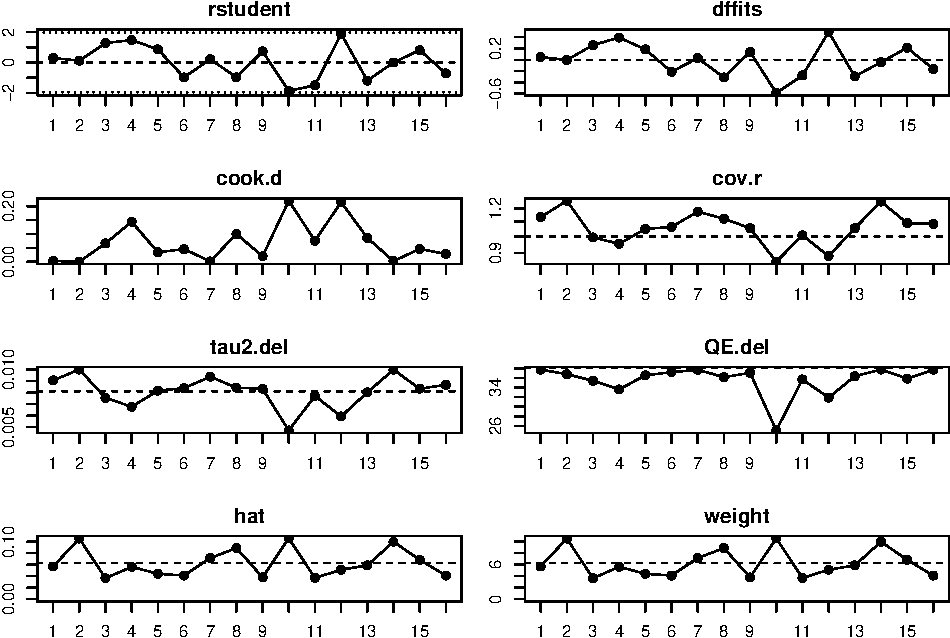
\includegraphics{Meta-analysis_files/figure-latex/unnamed-chunk-11-1.pdf}
\caption{\label{fig:unnamed-chunk-11}Diagnóstico de influencia. Estudios particularmente influyentes serían representados con un punto rojo. En este caso, no hay ningún estudio que se considere demasiado influyente, por lo que podemos estar tranquilos con nuestro meta-análisis.}
\end{figure}

\hypertarget{forest-plot-diagrama-de-bosque}{%
\subsection{\texorpdfstring{\emph{Forest plot} (diagrama de bosque)}{Forest plot (diagrama de bosque)}}\label{forest-plot-diagrama-de-bosque}}

Para hacer un diagrama de bosque (\emph{forest plot}) con \href{https://www.metafor-project.org/doku.php}{\texttt{metafor}} resumiendo nuestro meta-análisis, solo tenemos que usar la función \texttt{forest}, usando como argumento el objeto al que asignamos los resultados de nuestro meta-análisis (\texttt{res}).

\begin{Shaded}
\begin{Highlighting}[]
\FunctionTok{forest}\NormalTok{(res)}
\end{Highlighting}
\end{Shaded}

\begin{figure}
\centering
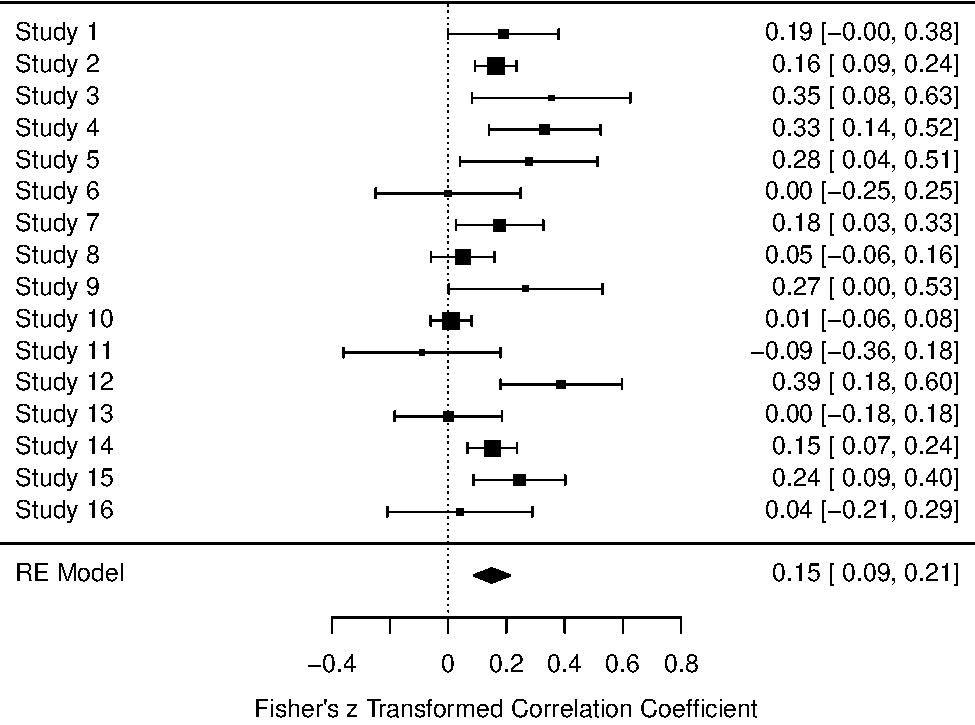
\includegraphics{Meta-analysis_files/figure-latex/for-plot1-1.pdf}
\caption{\label{fig:for-plot1}Forest plot básico de \href{https://www.metafor-project.org/doku.php}{metafor}. Para cada estudio meta-analizado, tenemos el efecto (correlación, en este caso en valores \emph{z} de Fisher), así como sus intervalos de confianza entre paréntesis cuadrados. Esta misma información está representada gráficamente, con los cuadrados representando el efecto de cada estudio así como sus intervalos de confianza, y el tamaño de muestra (representado por el tamaño del cuadrado). Bajo estos resultados, tenemos nuestro meta-análisis, con el mismo formato en texto, pero representando el efecto y sus intervalos de confianza con un diamante.}
\end{figure}

Como se puede ver en las Figuras \ref{fig:for-plot1}, \ref{fig:for-plot2} y \ref{fig:for-plot3} (que son versiones del mismo \emph{forest plot}), no es una sorpresa que el análisis nos sugiera bastante heterogeneidad; las correlaciones encontradas entre los diferentes estudios varían mucho (están entre -0.09 y 0.37), y aunque son positivas en la mayoría de los casos (en algunos claramente positivas), en algunos son prácticamente 0 o incluso negativas.

Para una versión más completa y anotada, también usando el \emph{plot} básico de \href{https://www.metafor-project.org/doku.php}{\texttt{metafor}}, pero agregando encabezados de cada columna en español, nombres de los estudios meta-analizados (pegando las columnas \texttt{authors} y \texttt{year} separadas por una coma y un espacio: \texttt{paste(dat\$authors,\ dat\$year,\ sep\ =\ ",\ ")} como argumento \texttt{slab}) así como agregando una columna con los pesos dados a cada estudio, y detalles del modelo final (estas opciones están explicadas \href{https://search.r-project.org/CRAN/refmans/metafor/html/forest.rma.html}{acá}):

\begin{Shaded}
\begin{Highlighting}[]
\CommentTok{\# forest plot con anotaciones adicionales}
\FunctionTok{forest}\NormalTok{(res, }\AttributeTok{cex =} \FloatTok{0.75}\NormalTok{, }\AttributeTok{xlim =} \FunctionTok{c}\NormalTok{(}\SpecialCharTok{{-}}\FloatTok{1.6}\NormalTok{, }\FloatTok{1.6}\NormalTok{),}
       \AttributeTok{slab =} \FunctionTok{paste}\NormalTok{(dat}\SpecialCharTok{$}\NormalTok{authors, dat}\SpecialCharTok{$}\NormalTok{year, }\AttributeTok{sep =} \StringTok{", "}\NormalTok{),}
       \AttributeTok{showweights =} \ConstantTok{TRUE}\NormalTok{,}
       \AttributeTok{atransf =}\NormalTok{ transf.ztor, }
       \AttributeTok{xlab =} \StringTok{"Coeficiente de correlación transformado en z de Fisher"}\NormalTok{,}
       \AttributeTok{digits =} \FunctionTok{c}\NormalTok{(}\DecValTok{2}\NormalTok{,3L),}
       \AttributeTok{mlab =} \FunctionTok{bquote}\NormalTok{(}\FunctionTok{paste}\NormalTok{(}\StringTok{"Modelo EA: Q("}\NormalTok{, .(res}\SpecialCharTok{$}\NormalTok{k }\SpecialCharTok{{-}}\NormalTok{ res}\SpecialCharTok{$}\NormalTok{p), }\StringTok{") = "}\NormalTok{,}
\NormalTok{     .(}\FunctionTok{formatC}\NormalTok{(res}\SpecialCharTok{$}\NormalTok{QE, }\AttributeTok{digits=}\DecValTok{2}\NormalTok{, }\AttributeTok{format=}\StringTok{"f"}\NormalTok{)),}
     \StringTok{", p "}\NormalTok{, .(scales}\SpecialCharTok{::}\FunctionTok{pvalue}\NormalTok{(res}\SpecialCharTok{$}\NormalTok{pval)), }\StringTok{"; "}\NormalTok{, I}\SpecialCharTok{\^{}}\DecValTok{2}\NormalTok{, }\StringTok{" = "}\NormalTok{,}
\NormalTok{     .(}\FunctionTok{formatC}\NormalTok{(res}\SpecialCharTok{$}\NormalTok{I2, }\AttributeTok{digits=}\DecValTok{1}\NormalTok{, }\AttributeTok{format=}\StringTok{"f"}\NormalTok{)), }\StringTok{"\%"}\NormalTok{)))}
\CommentTok{\# agregar encabezados a las columnas (valores de X y Y deben ser ajustados)}
\NormalTok{op }\OtherTok{\textless{}{-}} \FunctionTok{par}\NormalTok{(}\AttributeTok{cex =} \FloatTok{0.8}\NormalTok{, }\AttributeTok{font=}\DecValTok{2}\NormalTok{) }
\FunctionTok{text}\NormalTok{(}\AttributeTok{x =} \SpecialCharTok{{-}}\FloatTok{1.6}\NormalTok{, }\AttributeTok{y =} \DecValTok{18}\NormalTok{, }\AttributeTok{labels =} \StringTok{"Autor(es), Año"}\NormalTok{, }\AttributeTok{pos =} \DecValTok{4}\NormalTok{)}
\FunctionTok{text}\NormalTok{(}\AttributeTok{x =} \DecValTok{0}\NormalTok{, }\AttributeTok{y =} \DecValTok{18}\NormalTok{, }\AttributeTok{labels =} \StringTok{"Efecto e IC"}\NormalTok{, }\AttributeTok{pos =} \DecValTok{4}\NormalTok{)}
\FunctionTok{text}\NormalTok{(}\AttributeTok{x =} \DecValTok{1}\NormalTok{, }\AttributeTok{y =} \DecValTok{18}\NormalTok{, }\AttributeTok{labels =} \StringTok{"Peso"}\NormalTok{, }\AttributeTok{pos =} \DecValTok{2}\NormalTok{)}
\FunctionTok{text}\NormalTok{(}\AttributeTok{x =} \FloatTok{1.6}\NormalTok{, }\AttributeTok{y =} \DecValTok{18}\NormalTok{, }\AttributeTok{labels =} \StringTok{"Corr. [95\% IC]"}\NormalTok{, }\AttributeTok{pos =} \DecValTok{2}\NormalTok{)}
\end{Highlighting}
\end{Shaded}

\begin{figure}
\centering
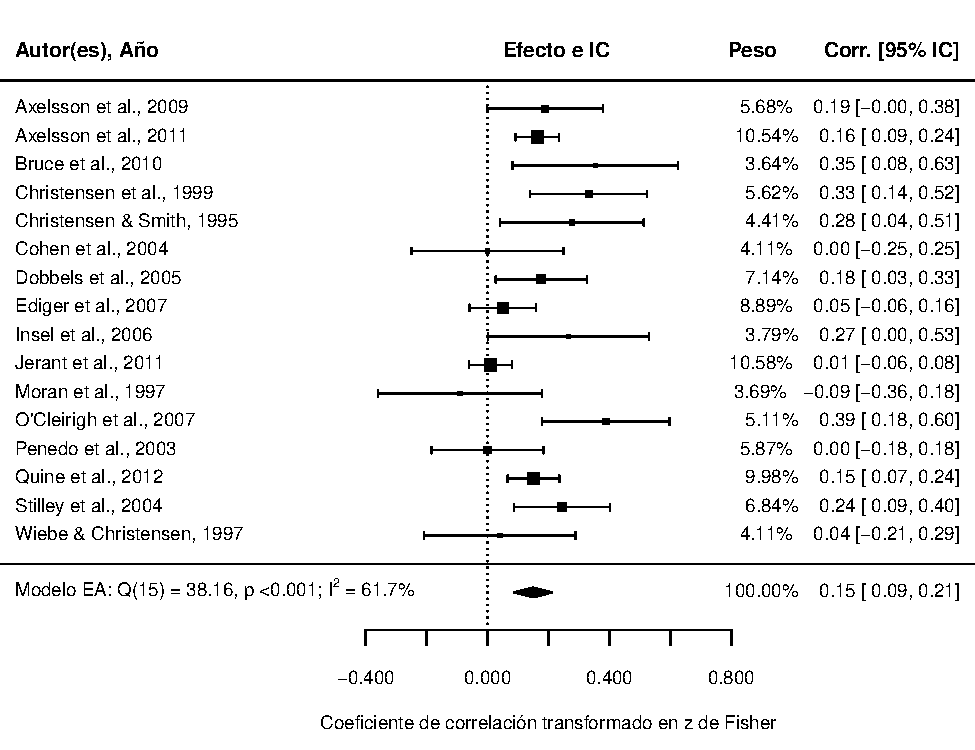
\includegraphics{Meta-analysis_files/figure-latex/for-plot2-1.pdf}
\caption{\label{fig:for-plot2}Forest plot anotado, creado con \href{https://www.metafor-project.org/doku.php}{metafor}. En esta versión agregué algunos encabezados en español, así como estadísticos generales del modelo de meta-análisis. Modelo EA se refiere al modelo meta-analizado, de efectos aleatorios.}
\end{figure}

O, para una incluso más sofisticada, se puede usar la función \href{https://cran.r-project.org/web/packages/metaviz/vignettes/metaviz.html\#creating-forest-plots-with-function-viz_forest}{\texttt{viz\_forest}} del paquete \href{https://cran.r-project.org/web/packages/metaviz/vignettes/metaviz.html}{\texttt{metaviz}}.

\begin{Shaded}
\begin{Highlighting}[]
\FunctionTok{library}\NormalTok{(metaviz)}

\CommentTok{\# A. Variante "classic" (no tiene que ser definida, pues es la opción por defecto)}
\FunctionTok{viz\_forest}\NormalTok{(res, }
           \AttributeTok{study\_labels =} \FunctionTok{paste}\NormalTok{(dat}\SpecialCharTok{$}\NormalTok{authors, dat}\SpecialCharTok{$}\NormalTok{year, }\AttributeTok{sep =} \StringTok{", "}\NormalTok{),}
           \AttributeTok{xlab =} \StringTok{"Correlación"}\NormalTok{, }
           \AttributeTok{annotate\_CI =} \ConstantTok{TRUE}\NormalTok{,}
           \AttributeTok{summary\_label =} \StringTok{"Resumen"}\NormalTok{,}
           \AttributeTok{text\_size =} \FloatTok{2.6}\NormalTok{,}
           \AttributeTok{x\_trans\_function =}\NormalTok{ tanh)}

\CommentTok{\# B. Variante "thick"}
\FunctionTok{viz\_forest}\NormalTok{(res, }
           \AttributeTok{study\_labels =} \FunctionTok{paste}\NormalTok{(dat}\SpecialCharTok{$}\NormalTok{authors, dat}\SpecialCharTok{$}\NormalTok{year, }\AttributeTok{sep =} \StringTok{", "}\NormalTok{),}
           \AttributeTok{xlab =} \StringTok{"Correlación"}\NormalTok{, }
           \AttributeTok{variant =} \StringTok{"thick"}\NormalTok{,}
           \AttributeTok{col =} \StringTok{"Greens"}\NormalTok{,}
           \AttributeTok{annotate\_CI =} \ConstantTok{TRUE}\NormalTok{,}
           \AttributeTok{summary\_label =} \StringTok{"Resumen"}\NormalTok{,}
           \AttributeTok{text\_size =} \FloatTok{2.6}\NormalTok{,}
           \AttributeTok{x\_trans\_function =}\NormalTok{ tanh)}

\CommentTok{\# C. Variante "rain"}
\FunctionTok{viz\_forest}\NormalTok{(res, }
           \AttributeTok{study\_labels =} \FunctionTok{paste}\NormalTok{(dat}\SpecialCharTok{$}\NormalTok{authors, dat}\SpecialCharTok{$}\NormalTok{year, }\AttributeTok{sep =} \StringTok{", "}\NormalTok{),}
           \AttributeTok{xlab =} \StringTok{"Correlación"}\NormalTok{, }
           \AttributeTok{variant =} \StringTok{"rain"}\NormalTok{,}
           \AttributeTok{col =} \StringTok{"Purples"}\NormalTok{,}
           \AttributeTok{annotate\_CI =} \ConstantTok{TRUE}\NormalTok{,}
           \AttributeTok{summary\_label =} \StringTok{"Resumen"}\NormalTok{,}
           \AttributeTok{text\_size =} \FloatTok{2.6}\NormalTok{,}
           \AttributeTok{x\_trans\_function =}\NormalTok{ tanh)}
\end{Highlighting}
\end{Shaded}

Con el código anterior genero las siguientes tres versiones del mismo \emph{forest plot} usando diferentes variantes y escalas de colores, y transformando de vuelta los coeficientes de \emph{z} de Fisher a \emph{r} de Pearson. Por supuesto, es cuestión de gusto cuál usar.

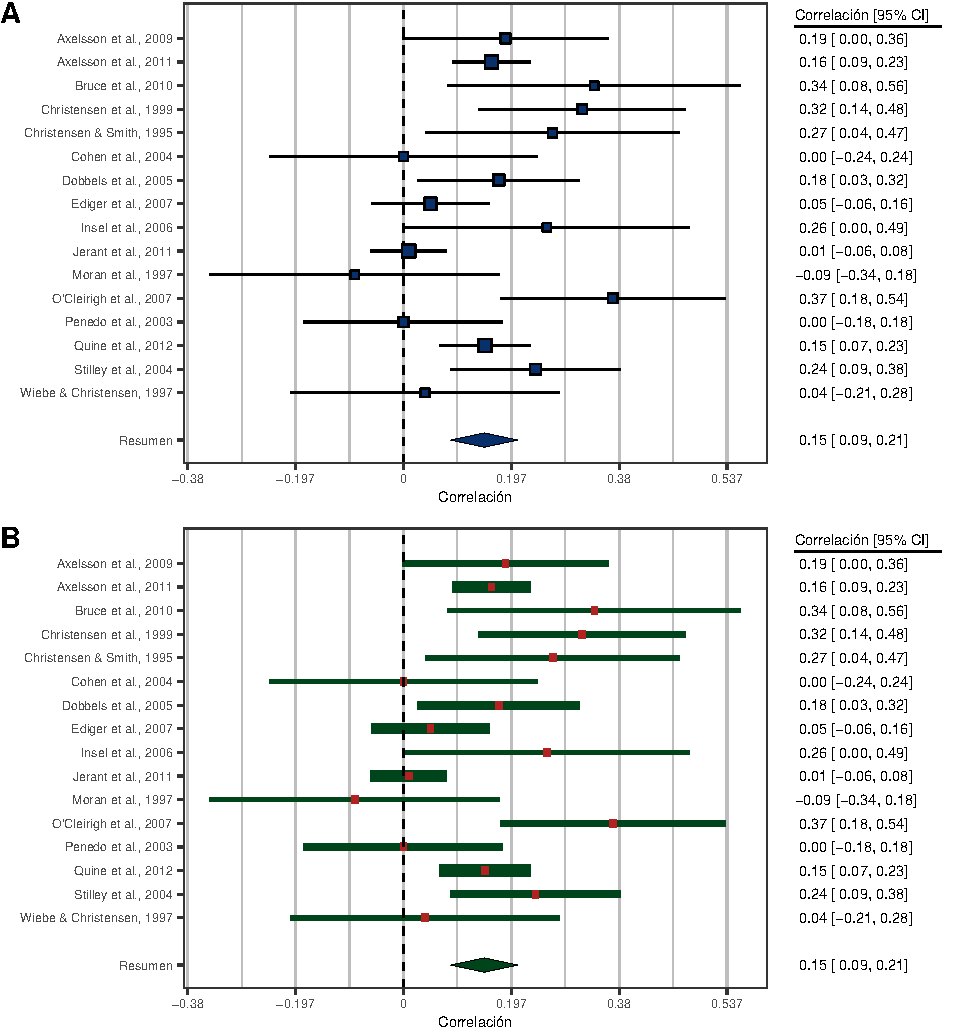
\includegraphics{Meta-analysis_files/figure-latex/for-plot3-1.pdf}

\begin{figure}
\centering
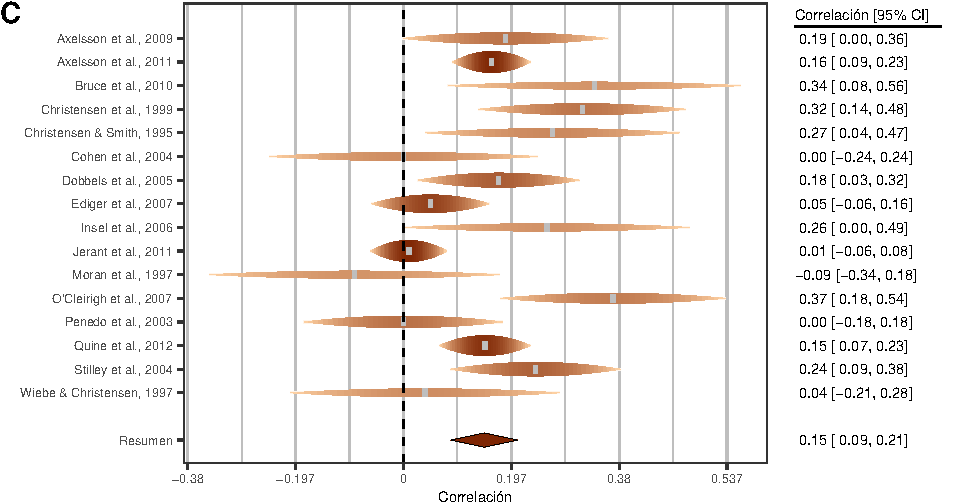
\includegraphics{Meta-analysis_files/figure-latex/for-plot3b-1.pdf}
\caption{\label{fig:for-plot3b}Variantes de forest plots creados con \href{https://cran.r-project.org/web/packages/metaviz/vignettes/metaviz.html}{metaviz}. \textbf{A.} Variante clásica (opción por defecto). \textbf{B.} Variante ``thick'' y escala de colores ``Greens''. \textbf{C.} Variante ``rain'' y escala de colores ``Purples''.}
\end{figure}

\hypertarget{funnel-plot-diagrama-de-embudo-y-sesgo-de-estudios-pequeuxf1os}{%
\subsection{\texorpdfstring{\emph{Funnel plot} (diagrama de embudo) y sesgo de estudios pequeños}{Funnel plot (diagrama de embudo) y sesgo de estudios pequeños}}\label{funnel-plot-diagrama-de-embudo-y-sesgo-de-estudios-pequeuxf1os}}

En este punto, es en donde más errores se cometen. Las pruebas más comunes para evaluar sesgos de publicación, son la evaluación de la asimatría en el \emph{funnel plot} (diagrama de embudo), y la regresión (o test) de Egger (\protect\hyperlink{ref-eggerBiasMetaanalysisDetected1997}{Egger et al., 1997}).

El principal error que la mayoría de los investigadores (meta-analistas) cometen, es que simplemente basándose en éstos métodos, concluyen que un meta-análisis tiene (o no) riesgo de sufrir de un sesgo de publicación. Sin embargo, estos métodos, no son pruebas exclusivas de sesgo de publicación, sino de sesgo de estudios de tamaño muestral pequeño (ver e.g. \protect\hyperlink{ref-schwarzerSmallStudyEffectsMetaAnalysis2015}{Schwarzer et al., 2015}), que pueden incluir sesgo de publicación, pero no se centran exclusivamente en éste.

A pesar de esto, tanto la regresión de Egger como el \emph{funnel plot}, son intersantes dado que el sesgo de estudios pequeños es importante.

\hypertarget{funnel-plot}{%
\subsubsection{\texorpdfstring{\emph{Funnel plot}}{Funnel plot}}\label{funnel-plot}}

Para crear un \emph{funnel plot} con \href{https://www.metafor-project.org/doku.php}{\texttt{metafor}}, de nuestro meta-análisis, solo tenemos que usar la función \texttt{funnel}, usando como argumento el objeto al que asignamos los resultados de nuestro meta-análisis (\texttt{res}).

\begin{Shaded}
\begin{Highlighting}[]
\FunctionTok{funnel}\NormalTok{(res)}
\end{Highlighting}
\end{Shaded}

\begin{figure}
\centering
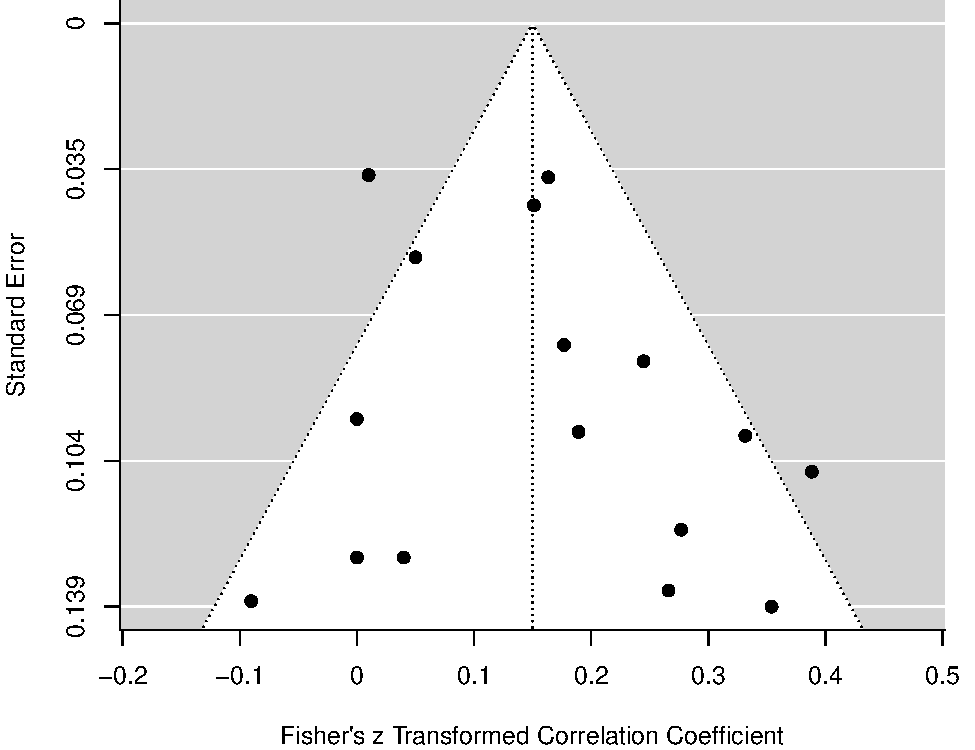
\includegraphics{Meta-analysis_files/figure-latex/funnel-plot1-1.pdf}
\caption{\label{fig:funnel-plot1}Funnel plot básico de \href{https://www.metafor-project.org/doku.php}{metafor}. Para cada estudio meta-analizado, tenemos el efecto (correlación, en este caso en valores \emph{z} de Fisher) en el eje \emph{X}, así como su error estándar en el eje \emph{Y}. La línea punteada vertical representa el efecto meta-analizado que hemos encontrado, así que podemos ver los estudios que encontraron un efecto mayor (derecha de la línea punteada) o menor (izquierda) de éste. A primera vista no parece haber mucha asimetría, pero es importante tener en cuenta que es un análisis muy subjetivo.}
\end{figure}

De nuevo, se puede usar el paquete \href{https://cran.r-project.org/web/packages/metaviz/vignettes/metaviz.html}{\texttt{metaviz}}, usando la función \href{https://cran.r-project.org/web/packages/metaviz/vignettes/metaviz.html\#creating-funnel-plots-with-viz_funnel}{\texttt{viz\_funnel}}. Hay muchas opciones, pero como ejemplo, usaré la versión por defecto, agregando solo la línea de la regressión de Egger (\texttt{egger\ =\ TRUE}; ver sección \ref{reg-egger}, a continuación), transformando los tamaños de efecto de regreso a \(r\) de Pearson (\texttt{x\_trans\_function\ =\ tanh}), y con los títulos de los ejes en español.

\begin{Shaded}
\begin{Highlighting}[]
\FunctionTok{viz\_funnel}\NormalTok{(res, }
           \AttributeTok{egger =} \ConstantTok{TRUE}\NormalTok{,}
           \AttributeTok{x\_trans\_function =}\NormalTok{ tanh,}
           \AttributeTok{ylab =} \StringTok{"Error estándar"}\NormalTok{,}
           \AttributeTok{xlab =} \StringTok{"Coeficiente de correlación"}\NormalTok{)}
\end{Highlighting}
\end{Shaded}

\begin{figure}
\centering
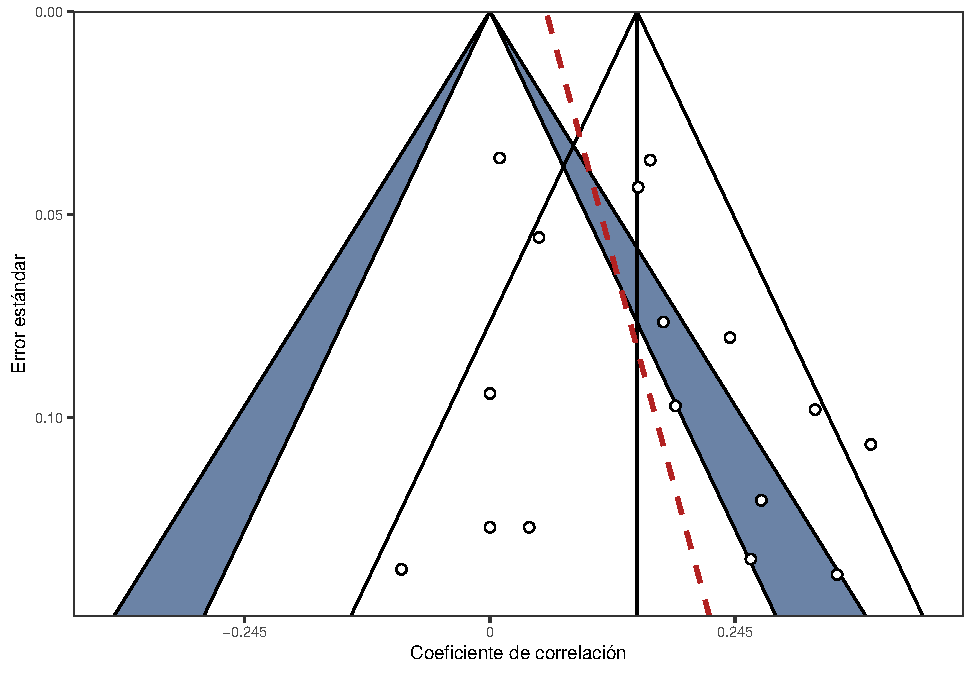
\includegraphics{Meta-analysis_files/figure-latex/funnel-plot2-1.pdf}
\caption{\label{fig:funnel-plot2}Funnel plot creado con \href{https://cran.r-project.org/web/packages/metaviz/vignettes/metaviz.html}{metaviz}. En azul, se representa el área donde estudios, según su error (y su tamaño de muestra), tendrían un efecto significativo al 5\% (i.e.~\(p\) \textgreater{} 0.05), y fuera de ésta, donde tendrían un efecto significativo al 1\% (i.e.~\(p\) \textgreater{} 0.01). La línea negra vertical representa el efecto meta-analizado, y el triángulo a partir de su inicio, el área donde se ubican los estudios que no se diferencian significativamente del resultado del meta-análisis. La línea roja punteada, representa la regresión de Egger.}
\end{figure}

Alternativamente, el paquete \href{https://cran.r-project.org/web/packages/metaviz/vignettes/metaviz.html}{\texttt{metaviz}} tiene la función \href{https://cran.r-project.org/web/packages/metaviz/vignettes/metaviz.html\#sunset-power-enhanced-funnel-plots}{\texttt{viz\_sunset}}, que permite además mostrar el poder estadístico (o potencia) de los estudios meta-analizados para detectar un efecto de interés mediante una prueba de Wald de dos colas. A continuación, muestro dos versiones de esta función. En ambos casos, agregué el efecto \emph{real} encontrado con el meta-análisis (\texttt{contours\ =\ TRUE}), y transformé los tamaños de efecto de regreso a \(r\) de Pearson (\texttt{x\_trans\_function\ =\ tanh}).

\begin{Shaded}
\begin{Highlighting}[]
\CommentTok{\# A. Escala de poder discreta}
\FunctionTok{viz\_sunset}\NormalTok{(res,}
           \AttributeTok{contours =} \ConstantTok{TRUE}\NormalTok{,}
           \AttributeTok{x\_trans\_function =}\NormalTok{ tanh,}
           \AttributeTok{ylab =} \StringTok{"Error estándar"}\NormalTok{,}
           \AttributeTok{xlab =} \StringTok{"Coeficiente de correlación"}\NormalTok{)}

\CommentTok{\# B. Escala de poder contínua}
\FunctionTok{viz\_sunset}\NormalTok{(res, }
           \AttributeTok{contours =} \ConstantTok{TRUE}\NormalTok{,}
           \AttributeTok{x\_trans\_function =}\NormalTok{ tanh, }
           \AttributeTok{power\_contours =} \StringTok{"continuous"}\NormalTok{,}
           \AttributeTok{ylab =} \StringTok{"Error estándar"}\NormalTok{,}
           \AttributeTok{xlab =} \StringTok{"Coeficiente de correlación"}\NormalTok{)}
\end{Highlighting}
\end{Shaded}

\begin{figure}
\centering
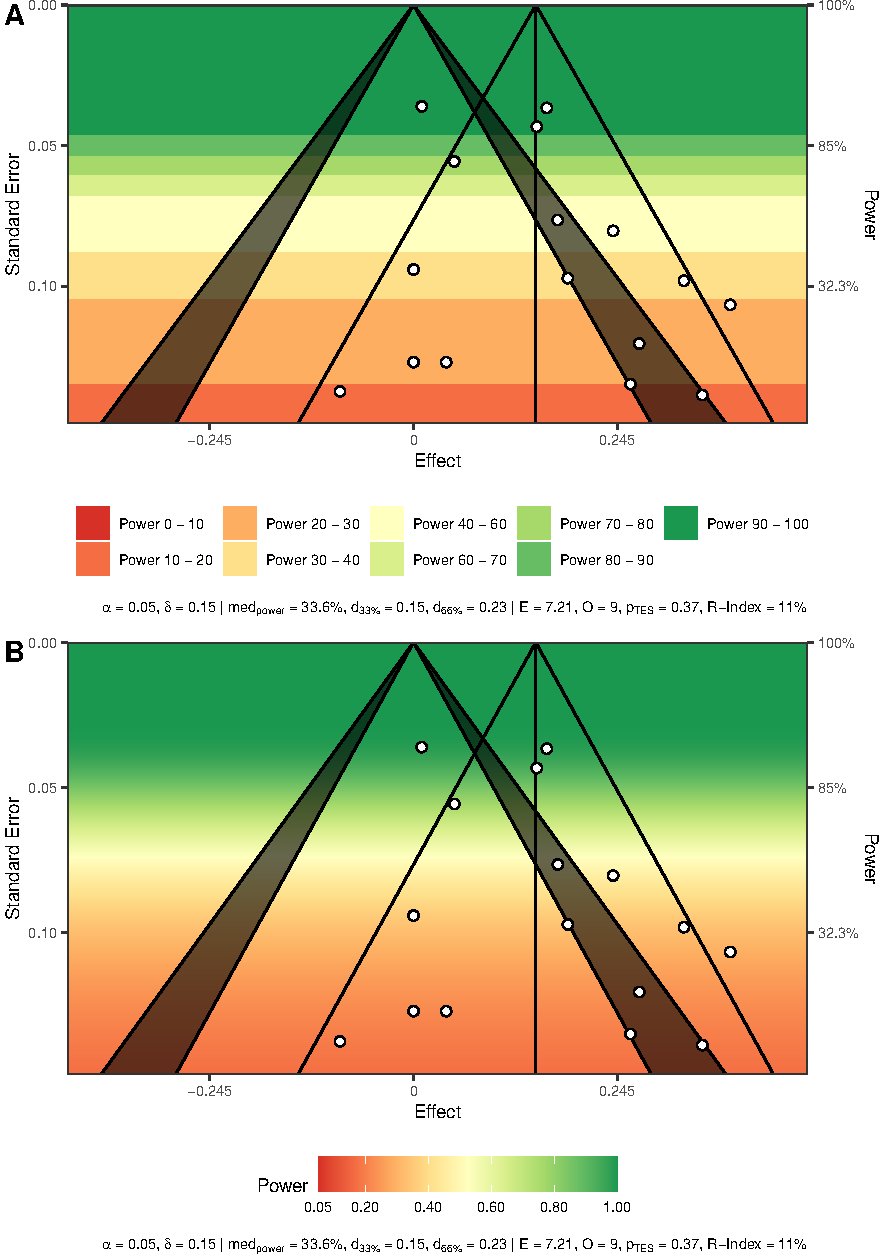
\includegraphics{Meta-analysis_files/figure-latex/funnel-plot3-1.pdf}
\caption{\label{fig:funnel-plot3}Dos versiones de funnel plot creados con \href{https://cran.r-project.org/web/packages/metaviz/vignettes/metaviz.html}{metaviz}, usando la función viz-sunset, que estima el poder de cada estudio para detectar un efecto de interés. \textbf{A.} Poder representado por bandas dicretas de color. \textbf{B.} Poder representado de manera contínua en una escala de color. En ambos casos, y tal como en la Fig. \ref{fig:funnel-plot2}, el efecto real está representado como una línea vertical, y el triángulo a partir de su inicio representa el área donde se ubican los estudios que no se diferencian significativamente del resultado del meta-análisis.}
\end{figure}

\hypertarget{reg-egger}{%
\subsubsection{Regresión de Egger}\label{reg-egger}}

Para hacer una prueba formal de sesgo de estudios pequeños, podemos hacer una prueba o regresión de Egger (\protect\hyperlink{ref-eggerBiasMetaanalysisDetected1997}{Egger et al., 1997}). En \href{https://www.metafor-project.org/doku.php}{\texttt{metafor}}, esto se hace con la función \texttt{regtest}, de nuevo usando como argumento el objeto al que asignamos el resultado de nuestro meta-análisis (\texttt{res}).

\begin{Shaded}
\begin{Highlighting}[]
\FunctionTok{regtest}\NormalTok{(res)}
\end{Highlighting}
\end{Shaded}

Como se puede ver, la prueba de Egger no muestra un resultado significativo (\texttt{z\ =\ 1.0216,\ p\ =\ 0.3070}).

\begin{footnotesize}
                \begin{Box2}{\texttt{Consola de R}}
                \begin{verbatim} 
Regression Test for Funnel Plot Asymmetry

Model:     mixed-effects meta-regression model
Predictor: standard error

Test for Funnel Plot Asymmetry: z = 1.0216, p = 0.3070
Limit Estimate (as sei -> 0):   b = 0.0790 (CI: -0.0686, 0.2266)
 \end{verbatim}
                \end{Box2}
                \end{footnotesize}

Con base en esto, y la inspección visual subjetiva del \emph{funnel plot}, muchos investigadores concluyen que no hay sesgo de publicación. Sin embargo, como mencioné antes, estas pruebas no se centran en el sesgo de publicación sino en el sesgo de estudios pequeños. En otras palabras, con base en esto, lo único que podemos concluir correctamente, es que no hay sesgo de estudios pequeños (más adelante, en la sección \ref{sesgo-pub}, explicaré cómo evaluar si hay sesgo de publicación).

\hypertarget{meta-anuxe1lisis-de-correlaciuxf3n-con-moderador}{%
\section{Meta-análisis de correlación con moderador}\label{meta-anuxe1lisis-de-correlaciuxf3n-con-moderador}}

\hypertarget{ejemplo-1-moderaciuxf3n-de-la-edad-promedio-de-los-participantes}{%
\subsection{Ejemplo 1: Moderación de la edad promedio de los participantes}\label{ejemplo-1-moderaciuxf3n-de-la-edad-promedio-de-los-participantes}}

Primero, y como ejemplo, vamos a ver si la edad (en nuestros datos, \texttt{meanage}) modera el resultado. Esto es importante, pues hay una enorme variación entre las edades medias de los participantes de los diferentes estudios\footnote{De hecho, mientras que en el estudio de Axelsson et al.~(2009) la edad promedio fue de 22, en el estudio de Jerant et al.~(2011) la edad promedio fue de 78.6.}, lo que podría moderar (afectar) la asociación entre diligencia (\emph{conscientiousness}) y adherencia a la medicación prescrita.

Para esto, de nuevo podemos usar la función \texttt{rma} de paquete \texttt{metafor} y de la misma manera que en la sección \ref{meta-cor}, pero agregando nuestra variable moderadora (\texttt{meanage}) al argumento \texttt{mods}. En este caso voy a asignar a un objeto llamado \texttt{res.modage}, para diferenciarlo del objeto \texttt{res} al que asigné el meta-análisis básico, sin moderadores.

\begin{Shaded}
\begin{Highlighting}[]
\NormalTok{res.modage }\OtherTok{\textless{}{-}} \FunctionTok{rma}\NormalTok{(}\AttributeTok{yi =}\NormalTok{ yi, }\AttributeTok{vi =}\NormalTok{ vi, }\AttributeTok{mods =} \SpecialCharTok{\textasciitilde{}}\NormalTok{meanage, }\AttributeTok{data =}\NormalTok{ dat)}
\end{Highlighting}
\end{Shaded}

Los resultados, son los siguientes:

\begin{Shaded}
\begin{Highlighting}[]
\NormalTok{res.modage}
\end{Highlighting}
\end{Shaded}

\begin{footnotesize}
                \begin{Box2}{\texttt{Consola de R}}
                \begin{verbatim} 
Mixed-Effects Model (k = 16; tau^2 estimator: REML)

tau^2 (estimated amount of residual heterogeneity):     0.0072 (SE = 0.0054)
tau (square root of estimated tau^2 value):             0.0846
I^2 (residual heterogeneity / unaccounted variability): 56.50%
H^2 (unaccounted variability / sampling variability):   2.30
R^2 (amount of heterogeneity accounted for):            11.76%

Test for Residual Heterogeneity:
QE(df = 14) = 30.9050, p-val = 0.0057

Test of Moderators (coefficient 2):
QM(df = 1) = 1.4286, p-val = 0.2320

Model Results:

         estimate      se     zval    pval    ci.lb   ci.ub 
intrcpt    0.2741  0.1090   2.5147  0.0119   0.0605  0.4877  * 
meanage   -0.0024  0.0020  -1.1952  0.2320  -0.0063  0.0015    

---
Signif. codes:  0 '***' 0.001 '**' 0.01 '*' 0.05 '.' 0.1 ' ' 1
 \end{verbatim}
                \end{Box2}
                \end{footnotesize}

Los resultados, que tienen la misma organización que los del análisis sin moderadores (sección \ref{meta-cor}) resultado nos muestra que, a pesar de la gran diferencia de edad entre estudios, la edad no tiene un efecto significativo, como se puede ver en la columna \texttt{pval} para el efecto de \texttt{meanage} (0.232).

\hypertarget{plot-mod}{%
\subsubsection{\texorpdfstring{\emph{Forest plot} y \emph{funnel plot}}{Forest plot y funnel plot}}\label{plot-mod}}

Por supuesto, de estos resultados también puedo crear \emph{forest plots} y \emph{funnel plots}, siguiendo los ejemplos y código de la sección \ref{meta-cor}.

Para el \emph{forest plot}, hago a continuación un ejemplo anotado y mejorado (tal como el ejemplo de la figura \ref{fig:for-plot2}), pero es importante tener en cuenta que esta opción no creará un resumen del meta-análisis.

\begin{Shaded}
\begin{Highlighting}[]
\CommentTok{\# forest plot con anotaciones adicionales}
\FunctionTok{forest}\NormalTok{(res.modage,  }\AttributeTok{cex =} \FloatTok{0.75}\NormalTok{, }\AttributeTok{xlim =} \FunctionTok{c}\NormalTok{(}\SpecialCharTok{{-}}\FloatTok{1.6}\NormalTok{, }\FloatTok{1.6}\NormalTok{),}
       \AttributeTok{slab =} \FunctionTok{paste}\NormalTok{(dat}\SpecialCharTok{$}\NormalTok{authors, dat}\SpecialCharTok{$}\NormalTok{year, }\AttributeTok{sep =} \StringTok{", "}\NormalTok{),}
       \AttributeTok{showweights =} \ConstantTok{TRUE}\NormalTok{,}
       \AttributeTok{atransf =}\NormalTok{ transf.ztor,}
       \AttributeTok{xlab =} \StringTok{"Coeficiente de correlación transformado en z de Fisher"}\NormalTok{,}
       \AttributeTok{digits =} \FunctionTok{c}\NormalTok{(}\DecValTok{2}\NormalTok{,3L))}
\CommentTok{\# agregar encabezados a las columnas (valores de X y Y deben ser ajustados)}
\NormalTok{op }\OtherTok{\textless{}{-}} \FunctionTok{par}\NormalTok{(}\AttributeTok{cex =} \FloatTok{0.8}\NormalTok{, }\AttributeTok{font=}\DecValTok{2}\NormalTok{)}
\FunctionTok{text}\NormalTok{(}\AttributeTok{x =} \SpecialCharTok{{-}}\FloatTok{1.6}\NormalTok{, }\AttributeTok{y =} \DecValTok{18}\NormalTok{, }\AttributeTok{labels =} \StringTok{"Autor(es), Año"}\NormalTok{, }\AttributeTok{pos =} \DecValTok{4}\NormalTok{)}
\FunctionTok{text}\NormalTok{(}\AttributeTok{x =} \DecValTok{0}\NormalTok{, }\AttributeTok{y =} \DecValTok{18}\NormalTok{, }\AttributeTok{labels =} \StringTok{"Efecto e IC"}\NormalTok{, }\AttributeTok{pos =} \DecValTok{4}\NormalTok{)}
\FunctionTok{text}\NormalTok{(}\AttributeTok{x =} \DecValTok{1}\NormalTok{, }\AttributeTok{y =} \DecValTok{18}\NormalTok{, }\AttributeTok{labels =} \StringTok{"Peso"}\NormalTok{, }\AttributeTok{pos =} \DecValTok{2}\NormalTok{)}
\FunctionTok{text}\NormalTok{(}\AttributeTok{x =} \FloatTok{1.6}\NormalTok{, }\AttributeTok{y =} \DecValTok{18}\NormalTok{, }\AttributeTok{labels =} \StringTok{"Corr. [95\% IC]"}\NormalTok{, }\AttributeTok{pos =} \DecValTok{2}\NormalTok{)}
\end{Highlighting}
\end{Shaded}

\begin{figure}
\centering
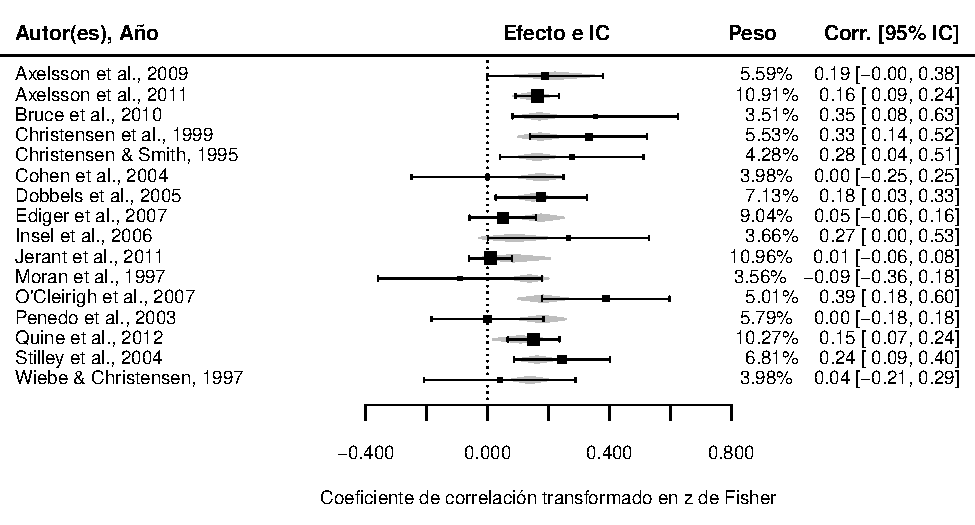
\includegraphics{Meta-analysis_files/figure-latex/for-plot-mod1-1.pdf}
\caption{\label{fig:for-plot-mod1}Forest plot básico de \href{https://www.metafor-project.org/doku.php}{metafor}, para un meta-análisis incluyendo la edad promedio de los participantes como moderador. En la ilustración gráfica, además de los efectos originales, se puede ver el efecto de cada estudio estimado cuando se incluye el moderador como polígonos (diamantes) de color gris. Sin embargo, ya no obtenemos una fila al final representando el efecto promediado del meta-análisis, ya que no tenemos un solo efecto.}
\end{figure}

Es importante tener en cuenta que la función \href{https://cran.r-project.org/web/packages/metaviz/vignettes/metaviz.html\#creating-forest-plots-with-function-viz_forest}{\texttt{viz\_forest}} del paquete \href{https://cran.r-project.org/web/packages/metaviz/vignettes/metaviz.html}{\texttt{metaviz}} tendrá problemas para crear un \emph{forest plot} de un meta-análisis con moderadores).

De manera similar, podemos obtener un \emph{funnel plot} de nuestro meta-análisis con moderador, pero éste nos mostrará, en vez de los coeficientes de correlación (transformados a \(z\) de Fisher), los valores residuales de cada estudio (es decir, qué tanto se alejan del resultado de nuestro meta-análisis):

\begin{Shaded}
\begin{Highlighting}[]
\FunctionTok{funnel}\NormalTok{(res.modage)}
\end{Highlighting}
\end{Shaded}

\begin{figure}
\centering
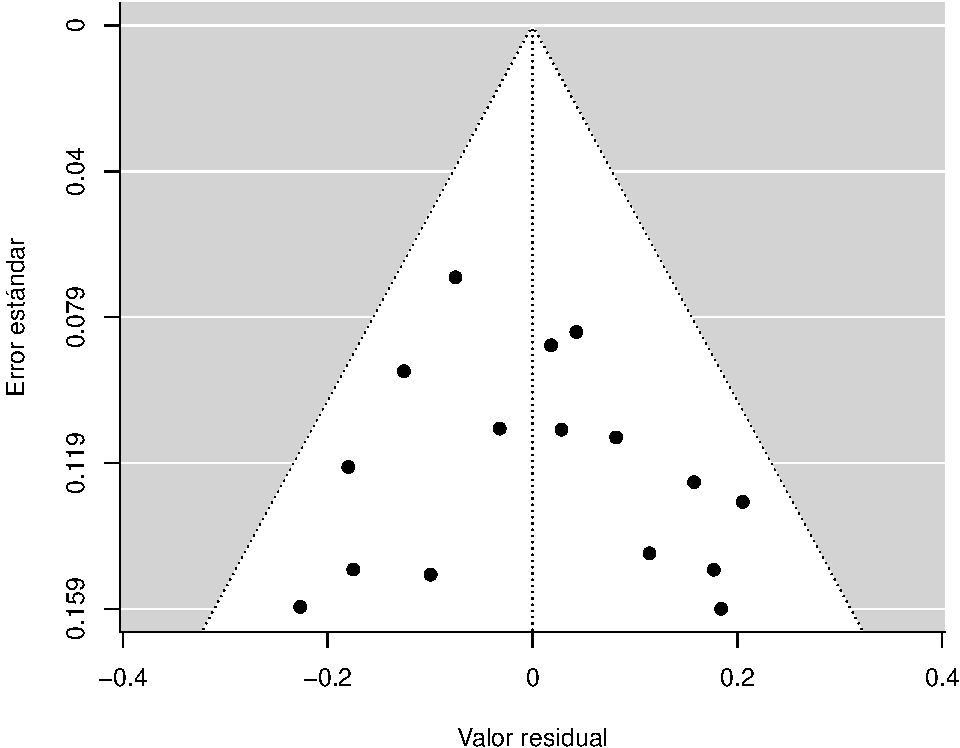
\includegraphics{Meta-analysis_files/figure-latex/funnel-plot-mod1-1.pdf}
\caption{\label{fig:funnel-plot-mod1}Funnel plot básico de \href{https://www.metafor-project.org/doku.php}{metafor}, para un meta-análisis incluyendo la edad promedio de los participantes como moderador. La línea punteada vertical representa el efecto meta-analizado que hemos encontrado, así que podemos ver los estudios que encontraron un efecto mayor (derecha de la línea punteada) o menor (izquierda) de éste.}
\end{figure}

\hypertarget{ejemplo-2-moderaciuxf3n-de-la-calidad-de-los-estudios-meta-analizados}{%
\subsection{Ejemplo 2: Moderación de la calidad de los estudios meta-analizados}\label{ejemplo-2-moderaciuxf3n-de-la-calidad-de-los-estudios-meta-analizados}}

La base de datos con tiene una medida de calidad metodológica de los estudios (variable \texttt{quality}). Dicha calidad, también podría moderar la asociación entre diligencia (\emph{conscientiousness}) y adherencia a la medicación prescrita. Siguiendo los mismos pasos, puedo hacer éste análisis, pero voy a asignar este meta-análisis a un objeto llamado \texttt{res.modq} para diferenciarlo de los demás.

\begin{Shaded}
\begin{Highlighting}[]
\NormalTok{res.modq }\OtherTok{\textless{}{-}} \FunctionTok{rma}\NormalTok{(}\AttributeTok{yi =}\NormalTok{ yi, }\AttributeTok{vi =}\NormalTok{ vi, }\AttributeTok{mods =} \SpecialCharTok{\textasciitilde{}}\NormalTok{quality, }\AttributeTok{data =}\NormalTok{ dat)}
\NormalTok{res.modq}
\end{Highlighting}
\end{Shaded}

\begin{footnotesize}
                \begin{Box2}{\texttt{Consola de R}}
                \begin{verbatim} 
Mixed-Effects Model (k = 16; tau^2 estimator: REML)

tau^2 (estimated amount of residual heterogeneity):     0.0078 (SE = 0.0057)
tau (square root of estimated tau^2 value):             0.0884
I^2 (residual heterogeneity / unaccounted variability): 57.79%
H^2 (unaccounted variability / sampling variability):   2.37
R^2 (amount of heterogeneity accounted for):            3.73%

Test for Residual Heterogeneity:
QE(df = 14) = 30.4205, p-val = 0.0067

Test of Moderators (coefficient 2):
QM(df = 1) = 0.6393, p-val = 0.4240

Model Results:

         estimate      se     zval    pval    ci.lb   ci.ub 
intrcpt    0.2082  0.0796   2.6149  0.0089   0.0521  0.3643  ** 
quality   -0.0312  0.0391  -0.7995  0.4240  -0.1078  0.0453     

---
Signif. codes:  0 '***' 0.001 '**' 0.01 '*' 0.05 '.' 0.1 ' ' 1
 \end{verbatim}
                \end{Box2}
                \end{footnotesize}

De nuevo, encontramos que éste moderador (\texttt{quality}), al igual que la edad promedio (\texttt{meanage}), no tiene un efecto significativo, como se puede ver en la columna \texttt{pval} para el efecto de \texttt{quality} (0.424).

Por supuesto, \emph{forest plots} y \emph{funnel plots} pueden ser creados, tal y como describí en la sección \ref{plot-mod}.

\hypertarget{ejemplo-3-moderaciuxf3n-de-las-controles-usados-en-cada-estudio-meta-analizado}{%
\subsection{Ejemplo 3: Moderación de las controles usados en cada estudio meta-analizado}\label{ejemplo-3-moderaciuxf3n-de-las-controles-usados-en-cada-estudio-meta-analizado}}

Como último ejemplo, voy a mirar si el hecho de que los estudios tengan variables que fueron controladas, modera la asociación entre diligencia (\emph{conscientiousness}) y adherencia a la medicación prescrita. Siguiendo los mismos pasos, voy hacer éste análisis, pero voy a asignar este meta-análisis a un objeto llamado \texttt{res.mes}. Son embargo, dado que la variable que contiene esta información (\texttt{controls}) es un factor, pero no está definido como tal, debo hacerlo en la usando la función \texttt{factor} al ingresar el argumento \texttt{mods} (i.e.~\texttt{mods\ =\ \textasciitilde{}factor(controls)}).

\begin{Shaded}
\begin{Highlighting}[]
\NormalTok{res.mes }\OtherTok{\textless{}{-}} \FunctionTok{rma}\NormalTok{(}\AttributeTok{yi =}\NormalTok{ yi, }\AttributeTok{vi =}\NormalTok{ vi, }\AttributeTok{mods =} \SpecialCharTok{\textasciitilde{}}\FunctionTok{factor}\NormalTok{(controls), }\AttributeTok{data =}\NormalTok{ dat)}
\NormalTok{res.mes}
\end{Highlighting}
\end{Shaded}

\begin{footnotesize}
                \begin{Box2}{\texttt{Consola de R}}
                \begin{verbatim} 
Mixed-Effects Model (k = 16; tau^2 estimator: REML)

tau^2 (estimated amount of residual heterogeneity):     0.0000 (SE = 0.0015)
tau (square root of estimated tau^2 value):             0.0002
I^2 (residual heterogeneity / unaccounted variability): 0.00%
H^2 (unaccounted variability / sampling variability):   1.00
R^2 (amount of heterogeneity accounted for):            100.00%

Test for Residual Heterogeneity:
QE(df = 14) = 18.0370, p-val = 0.2051

Test of Moderators (coefficient 2):
QM(df = 1) = 20.1221, p-val < .0001

Model Results:

                      estimate      se    zval    pval    ci.lb   ci.ub 
intrcpt                 0.0167  0.0296  0.5635  0.5731  -0.0413  0.0746      
factor(controls)none    0.1621  0.0361  4.4858  <.0001   0.0913  0.2329  *** 

---
Signif. codes:  0 '***' 0.001 '**' 0.01 '*' 0.05 '.' 0.1 ' ' 1
 \end{verbatim}
                \end{Box2}
                \end{footnotesize}

En éste caso, a diferencia de los ejemplos de moderación anteriores, la variable moderadora (\texttt{controls}) sí tiene un efecto significativo, como se puede ver en la columna \texttt{pval} para el efecto de \texttt{factor(controls)none} (\textless0.001), y en los asteriscos que aparecen al final de esa fila (\texttt{***}).

Por supuesto, \emph{forest plots} y \emph{funnel plots} pueden ser creados, tal y como describí en la sección \ref{plot-mod}.

\hypertarget{sesgo-pub}{%
\section{\texorpdfstring{Sesgo de publicación (\emph{publication bias})}{Sesgo de publicación (publication bias)}}\label{sesgo-pub}}

Para determinar el sesgo de publicación, se puede usar la función \texttt{weightfunct} del paquete \texttt{\{weightr\}}, que nos permite ``estimar tanto el modelo de función de peso para el sesgo de publicación que se publicó originalmente en Vevea y Hedges (\protect\hyperlink{ref-veveaGeneralLinearModel1995}{1995}) como la versión modificada presentada en Vevea y Woods (\protect\hyperlink{ref-veveaPublicationBiasResearch2005}{2005})'', como se describe en la \href{https://www.rdocumentation.org/packages/weightr/versions/2.0.2/topics/weightfunct}{documentación} de la función \texttt{weightfunct}.

\begin{Shaded}
\begin{Highlighting}[]
\FunctionTok{library}\NormalTok{(weightr)}
\end{Highlighting}
\end{Shaded}

En este caso, usaré esta función, asignando el resultado a un objeto que llamaré \texttt{wf}.

\begin{Shaded}
\begin{Highlighting}[]
\NormalTok{wf }\OtherTok{\textless{}{-}} \FunctionTok{weightfunct}\NormalTok{(}\AttributeTok{effect =}\NormalTok{ dat}\SpecialCharTok{$}\NormalTok{yi, }\AttributeTok{v =}\NormalTok{ dat}\SpecialCharTok{$}\NormalTok{vi, }\AttributeTok{table =} \ConstantTok{TRUE}\NormalTok{)}
\NormalTok{wf}
\end{Highlighting}
\end{Shaded}

\begin{footnotesize}
                \begin{Box2}{\texttt{Consola de R}}
                \begin{verbatim} 
Unadjusted Model (k = 16):

tau^2 (estimated amount of total heterogeneity): 0.0070 (SE = 0.0051)
tau (square root of estimated tau^2 value):  0.0834

Test for Heterogeneity:
Q(df = 15) = 38.1595, p-val = 0.001436053

Model Results:

          estimate std.error z-stat      p-val   ci.lb  ci.ub
Intercept   0.1486   0.03073  4.835 1.3288e-06 0.08837 0.2088

Adjusted Model (k = 16):

tau^2 (estimated amount of total heterogeneity): 0.0056 (SE = 0.0045)
tau (square root of estimated tau^2 value):  0.0750

Test for Heterogeneity:
Q(df = 15) = 38.1595, p-val = 0.001436053

Model Results:

              estimate std.error z-stat    p-val    ci.lb  ci.ub
Intercept      0.09153   0.04464  2.050 0.040341  0.00403 0.1790
0.025 < p < 1  0.24121   0.20122  1.199 0.230626 -0.15317 0.6356

Likelihood Ratio Test:
X^2(df = 1) = 2.98493, p-val = 0.084043

Number of Effect Sizes per Interval:

                     Frequency
p-values <0.025              9
0.025 < p-values < 1         7
 \end{verbatim}
                \end{Box2}
                \end{footnotesize}

\hypertarget{referencias}{%
\section*{Referencias}\label{referencias}}
\addcontentsline{toc}{section}{Referencias}

\hypertarget{refs}{}
\begin{CSLReferences}{1}{0}
\leavevmode\vadjust pre{\hypertarget{ref-borensteinIdentifyingQuantifyingHeterogeneity2009}{}}%
Borenstein, M., Hedges, L. V., Higgns, J. P. T., \& Rothstein, H. R. (2009). Identifying and {Quantifying Heterogeneity}. In \emph{Introduction to {Meta}-{Analysis}} (pp. 107--125). Wiley. \url{https://doi.org/10.1002/9780470743386.ch16}

\leavevmode\vadjust pre{\hypertarget{ref-eggerBiasMetaanalysisDetected1997}{}}%
Egger, M., Smith, G. D., Schneider, M., \& Minder, C. (1997). Bias in meta-analysis detected by a simple, graphical test. \emph{BMJ}, \emph{315}(7109), 629--634. \url{https://doi.org/10.1136/bmj.315.7109.629}

\leavevmode\vadjust pre{\hypertarget{ref-fisherRobumetaRpackageRobust2015}{}}%
Fisher, Z., \& Tipton, E. (2015). Robumeta: {An R}-package for robust variance estimation in meta-analysis. \emph{arXiv:1503.02220 {[}Stat{]}}. \url{https://arxiv.org/abs/1503.02220}

\leavevmode\vadjust pre{\hypertarget{ref-leongomezMetaanalysis2021}{}}%
Leongómez, J. D. (2021). \emph{Hacer meta-análisis en jamovi es muy fácil}. {[}Archivo de {Vídeo}{]}. YouTube. \url{https://youtu.be/ntBbkOn9D_o}.

\leavevmode\vadjust pre{\hypertarget{ref-molloy2013}{}}%
Molloy, G. J., O'Carroll, R. E., \& Ferguson, E. (2013). Conscientiousness and Medication Adherence: A Meta-analysis. \emph{Annals of Behavioral Medicine}, \emph{47}(1), 92--101. \url{https://doi.org/10.1007/s12160-013-9524-4}

\leavevmode\vadjust pre{\hypertarget{ref-quintanaHowPerformMetaanalysis2021}{}}%
Quintana, D. S. (2021). \emph{How to perform a meta-analysis in {R}}. {[}Archivo de {Vídeo}{]}. YouTube. \url{https://youtu.be/lH4VZMTEZSc}.

\leavevmode\vadjust pre{\hypertarget{ref-schwarzerSmallStudyEffectsMetaAnalysis2015}{}}%
Schwarzer, G., Carpenter, J. R., \& Rücker, G. (2015). Small-{Study Effects} in {Meta}-{Analysis}. In G. Schwarzer, J. R. Carpenter, \& G. Rücker (Eds.), \emph{Meta-{Analysis} with {R}} (pp. 107--141). {Springer International Publishing}. \url{https://doi.org/10.1007/978-3-319-21416-0_5}

\leavevmode\vadjust pre{\hypertarget{ref-veveaGeneralLinearModel1995}{}}%
Vevea, J. L., \& Hedges, L. V. (1995). A general linear model for estimating effect size in the presence of publication bias. \emph{Psychometrika}, \emph{60}(3), 419--435. \url{https://doi.org/10.1007/BF02294384}

\leavevmode\vadjust pre{\hypertarget{ref-veveaPublicationBiasResearch2005}{}}%
Vevea, J. L., \& Woods, C. M. (2005). Publication bias in research synthesis: Sensitivity analysis using a priori weight functions. \emph{Psychological Methods}, \emph{10}(4), 428--443. \url{https://doi.org/10.1037/1082-989X.10.4.428}

\leavevmode\vadjust pre{\hypertarget{ref-viechtbauer2010}{}}%
Viechtbauer, W. (2010). Conducting Meta-Analyses in {R} with the metafor Package. \emph{Journal of Statistical Software}, \emph{36}(3). \url{https://doi.org/10.18637/jss.v036.i03}

\end{CSLReferences}

\end{document}
